% Springer Nature manuscript format (vendored under LPPL for a self-contained archive).
\RequirePackage{xr-hyper}
\documentclass[pdflatex,referee]{template/sn-jnl}
% A4 review layout: use the page instead of the class's small-format text block.
% Keep review line spacing; limit whitespace around figures and the title.
\geometry{reset,a4paper,left=22mm,right=24mm,top=20mm,bottom=22mm,
          bindingoffset=0mm,footskip=10mm}
\raggedbottom
\setlength{\floatsep}{10pt plus 2pt minus 2pt}
\setlength{\textfloatsep}{10pt plus 2pt minus 2pt}
\setlength{\intextsep}{10pt plus 2pt minus 2pt}
\renewcommand{\topfraction}{.95}
\renewcommand{\bottomfraction}{.90}
\renewcommand{\textfraction}{.05}
\renewcommand{\floatpagefraction}{.80}
\makeatletter
% Float-only pages start at the top instead of being vertically centred.
\setlength{\@fptop}{0pt}
\setlength{\@fpsep}{10pt plus 2pt minus 2pt}
\usepackage{etoolbox}
\patchcmd{\@maketitle}{\vskip21pt}{\vskip0pt}{}{}
% The class also inserts an empty opening box and an unused article-type row.
\patchcmd{\@maketitle}{\newpage\null}{\newpage}{}{\PackageError{synkit-layout}{Cannot remove title opening box}{Check the class title definition.}}
\patchcmd{\@maketitle}{{\hbox to \textwidth{{\Artcatfont\ArtType\hfill}\par}}}{}{}{\PackageError{synkit-layout}{Cannot remove unused article-type row}{Check the class title definition.}}
\patchcmd{\@maketitle}{\vskip20pt}{\vskip0pt}{}{\PackageError{synkit-layout}{Cannot remove title padding}{Check the class title definition.}}
\pretocmd{\Titlefont}{\def\baselinestretch{1}}{}{}
\patchcmd{\@maketitle}{\vskip36pt}{\vskip12pt}{}{}
\makeatother

% Capability marks for the software-scope table.  Defined here, in the shared
% preamble, because xr-hyper imports main.aux (and its caption) into the SI.
% Shape carries the meaning; the marks are distinguishable without colour.
\newcommand{\yes}{\ensuremath{\checkmark}}
\newcommand{\no}{\ensuremath{\times}}
\newcommand{\pmark}{\ensuremath{(\checkmark)}}
\newcommand{\rot}[1]{\rotatebox[origin=l]{90}{#1}}


\usepackage[T1]{fontenc}
\usepackage{lmodern}
\usepackage{xspace}
\usepackage{graphicx}
\usepackage{xcolor}
\usepackage{booktabs}
\usepackage{microtype}
\usepackage{amsmath,amssymb}
\usepackage{mathrsfs}
\usepackage{subcaption}
\usepackage{float}
\usepackage{tabularx}
\usepackage{longtable}
\usepackage{array}
\usepackage{multirow}
\usepackage{pdflscape}
\usepackage{adjustbox}
\usepackage{enumitem}
\usepackage{siunitx}
\usepackage[version=4]{mhchem}
\usepackage{chemfig}
\usepackage{tikz}
\usepackage{pgfplots}

% Evidence figures are regenerated from JSON, and the glycolysis diagram uses TikZ.
% Shared figure styling is defined in paper_layout.tex.
\usepackage[numbers,square]{natbib}
\bibliographystyle{template/spbasic_u}

\newcommand{\synkit}{\texttt{SynKit}\xspace}
\newcommand{\synkitcrn}{\texttt{SynKit CRN}\xspace}
\hyphenation{SynKit Bio-in-for-mat-ics Reactome Wiki-Pathways}

% Help TeX avoid underfull lines in justified text
\emergencystretch=2em
\tolerance=2000
\hbadness=2000

\usepackage{hyperref}
\hypersetup{
  bookmarksdepth=2,
  colorlinks=true,
  linkcolor=blue,
  citecolor=blue,
  filecolor=blue,
  urlcolor=blue,
  anchorcolor=blue,
  pdfauthor={Thanh-An Pham and Tieu-Long Phan}
}

\externaldocument[supp:]{SI/si}

\begin{document}

\title[On The Conservation Laws and Pathway Realizability]{On The Conservation Laws and Pathway Realizability\hb of Biochemical Reaction Networks}

\author[1]{\fnm{Thanh-An} \sur{Pham}}\email{thanh-an.pham@uni-leipzig.de}
\author*[1,2]{\fnm{Tieu-Long} \sur{Phan}}\email{tieu@bioinf.uni-leipzig.de}

\affil[1]{\orgdiv{Bioinformatics Group, Department of Computer Science \& Interdisciplinary Center for Bioinformatics \& School for Embedded and Composite Artificial Intelligence (SECAI)}, \orgname{Leipzig University}, \orgaddress{\street{H{\"a}rtelstra{\ss}e 16--18}, \postcode{D-04107}, \city{Leipzig}, \country{Germany}}}
\affil[2]{\orgdiv{Department of Mathematics and Computer Science}, \orgname{University of Southern Denmark}, \orgaddress{\postcode{DK-5230}, \city{Odense M}, \country{Denmark}}}

% Generated numerical values shared with the supplement.
% BEGIN GENERATED: review-macros
% Generated from crn-review-experiments.json; do not edit.
\newcommand{\ReviewExhaustiveMilliseconds}{29.25}
\newcommand{\ReviewClosureMilliseconds}{0.63}
\newcommand{\ReviewRoundedFailures}{3}
\newcommand{\ReviewRatioSmall}{1.0}
\newcommand{\ReviewRatioLarge}{46.6}
\newcommand{\ReviewReversibleSiphonSeconds}{0.279}
\newcommand{\ReviewReversibleCanonicalSeconds}{0.343}
\newcommand{\ReviewReversibleMoietySeconds}{1.02}
\newcommand{\ReviewReversibleRankSeconds}{2.15}
\newcommand{\ReviewRandomSiphonSeconds}{0.113}
\newcommand{\ReviewRandomMoietySeconds}{0.0789}
\newcommand{\ReviewBioModelSiphonSeconds}{0.0235}
\newcommand{\ReviewBioModelMoietySeconds}{2.15}
\newcommand{\ReviewFormoseGenerationSeconds}{0.0177}
% END GENERATED: review-macros


% BEGIN GENERATED: dpo-generation-macros
% Generated from formose-expansion/dpo/comparison.json.
\newcommand{\DpoNativeFourSeconds}{0.0177}
\newcommand{\DpoNativeFiveSeconds}{0.0417}
\newcommand{\DpoNativeSixSeconds}{1.36}
\newcommand{\DpoModSixSeconds}{1.57}
\newcommand{\DpoMolfoundrySixSeconds}{11.8}
% END GENERATED: dpo-generation-macros

% BEGIN GENERATED: glycolysis-macros
% Generated by glycolysis_analysis.py; do not edit by hand.
\def\GlySpecies{14}
\def\GlyReactions{15}
\def\GlyComplexes{16}
\def\GlyLinkage{4}
\def\GlyRank{11}
\def\GlyDeficiency{1}
\def\GlyMoieties{3}
\def\GlyBackboneSupport{11}
\def\GlySiphons{3}
\def\GlyUncovered{2}
\def\GlyCertificateLength{15}
\def\GlyExplored{30}
\def\GlyDepth{15}
\def\GlyUpperFirings{5}
\def\GlyLowerFirings{10}
\def\GlySplitStep{4}
\def\GlyTrajectory{0/1/2,1/1/2,2/1/2,3/1/2,4/2/2,5/2/2,6/2/2,7/2/2,8/2/2,9/2/2,10/2/2,11/2/2,12/2/2,13/2/2,14/2/2,15/2/2}
% END GENERATED: glycolysis-macros

\abstract{
\textbf{Background:} Conserved metabolite pools and substrate availability constrain biochemical pathways before kinetic parameters are known. The two are usually examined on different abstractions: conservation on the net stoichiometric matrix and feasibility on graphs or flux balances. Catalysts and recycled cofactors that appear identically on both sides of a reaction cancel from net stoichiometry despite being required for firing, so a reduction made for one analysis can invalidate another.

\textbf{Results:} We present the chemical reaction network (CRN) submodule of \synkit, an open-source Python toolkit with a C++ core. It builds networks from \texttt{KEGG} pathways, \texttt{SBML} models, and reaction rules into a unified representation keeping reactant and product incidences separate. On this representation it computes exact conservation laws, minimal semiflows and siphons, deficiency, and firing certificates determining whether a reaction multiset can execute from a finite inventory. Twelve reference networks match ground truth and agree with \texttt{CRNT4SBML} on eight shared structural quantities, whereas rounded floating-point bases yield invalid conservation vectors for three. Ten reaction-bearing \texttt{BioModels} entries, the largest with 504 species and 827 reactions, pass structural \texttt{SBML} round trips. At six iterations, formose rule expansion yields the same 10\,572 species and 11\,239 reactions as \texttt{M\O D} and \texttt{MolFoundry}. In \texttt{KEGG} glycolysis, net reduction of shared polyphosphate preserves the stoichiometric matrix but drops deficiency from one to zero and removes the donor requirement. A 15-step glucose-to-pyruvate certificate exists when currency metabolites are removed, whereas exhaustive search shows this flux is unrealizable from glucose alone when they are retained. In the formose network, the single conservation law reproduces carbon counts for all 37 species, yet inventories with the same six carbon atoms differ in supplying selected tetrose and hexose routes.

\textbf{Conclusions:} Conservation laws are necessary but insufficient for pathway execution, and participant retention, cofactor boundaries, and precursor multiplicities each alter structural and realizability conclusions. Analyzing these on one model with exact arithmetic and certificates makes modeling assumptions explicit and testable. Source code, recorded results, and reproducible analyses accompany the manuscript.
}
\keywords{Chemical reaction networks, chemical reaction network theory, Petri nets, conserved moieties, stoichiometry, pathway realizability, \texttt{SBML}}
\maketitle

\section{Background}
\label{sec:intro}

Curated databases such as \texttt{KEGG}~\cite{kanehisa2025kegg}, \texttt{Reactome}~\cite{ragueneau2026reactome}, and \texttt{WikiPathways}~\cite{agrawal2024wikipathways} catalog known metabolic pathways and biochemical reactions, while graph-transformation methods enumerate candidate reactions from molecular seeds and transformation rules~\cite{andersen2016mod}. Before assigning kinetic parameters, structural analyses clarify the behavioral constraints imposed by network topology. Specifically, researchers examine which metabolite pools are conserved by stoichiometric invariants~\cite{famili2003leftnullspace}, which qualitative dynamical bounds or multistationarity criteria are governed by reaction network structure~\cite{feinberg1987deficiency,gunawardena2003crnt}, and whether a candidate pathway is realizable from a finite substrate inventory~\cite{andersen2023realisability}.

Assessing these constraints simultaneously is difficult because each analysis relies on a different mathematical abstraction of the biochemical system. A species graph captures connectivity between metabolites but loses the joint requirement of multiple co-substrates~\cite{franzese2019hypergraph}. The net stoichiometric matrix records net changes in species abundance but omits participants that appear identically as reactants and products, such as catalysts or recycled cofactors. For example, a catalyzed reaction $A+C\to B+C$ and the uncatalyzed conversion $A\to B$ yield identical net columns in $\mathbf S$, yet only the first requires the catalyst $C$ to proceed, and the two define different reaction complexes that alter network deficiency. Similarly, a balanced reaction combination or a qualitatively reachable product does not establish that the reactions can proceed in an admissible sequence from a finite inventory~\cite{andersen2023realisability}. Representation choices during model import can therefore compromise the assumptions of another analysis.

Because of these distinct formulations, existing software packages specialize in separate subsets of analyses: \texttt{COBRApy}~\cite{ebrahim2013cobrapy} supports constraint-based flux analysis~\cite{orth2010fba,schuster1994efm}, \texttt{CRNT4SBML}~\cite{reyes2020crnt4sbml} evaluates deficiency and potential bistability, \texttt{M\O D}~\cite{andersen2016mod} explores rule-generated reaction spaces, \texttt{Tellurium}~\cite{choi2018tellurium} and \texttt{libRoadRunner}~\cite{welsh2023libroadrunner} simulate kinetic ODEs, and Petri-net methods provide pathway realizability certificates~\cite{zevedei2003topological,murata1989petri,andersen2023realisability}. Standard exchange formats such as \texttt{SBML}~\cite{hucka2003sbml} and \texttt{COMBINE}~\cite{bergmann2014combine}, alongside converters like \texttt{KEGGtranslator}~\cite{wrzodek2011keggtranslator}, facilitate model transfer. However, converting models between separate formats can inadvertently discard structural features, such as catalysts or boundary species, that specific analyses require.

Conserved pools and substrate sufficiency therefore need to be examined on the same underlying reaction model. In glycolysis~\cite{kanehisa2025kegg}, a route appears connected from glucose to pyruvate when cofactors are omitted, yet cannot proceed when ATP and redox cofactors are retained with finite initial pools. In a rule-generated formose network~\cite{butlerov1861formose}, every reaction may conserve carbon, yet a proposed pathway remains unrealizable if its reactions require more glycolaldehyde molecules than the initial precursor pool provides. In both cases, conservation laws alone cannot establish whether a reaction sequence is realizable from a specified finite inventory~\cite{andersen2023realisability}.

Here, we present the chemical reaction network (CRN) submodule of \synkit~\cite{phan2025synkit} to evaluate these constraints on a shared representation. By connecting \texttt{KEGG} pathway import, structural \texttt{SBML} exchange, and rule-based generation to exact conservation laws, deficiency theory, and Petri-net reachability, the toolkit tests whether reaction sequences can execute without discarding catalysts or cofactors. We validate the implementation across twelve reference networks against \texttt{CRNT4SBML}, verify structural round trips on ten \texttt{BioModels} entries, and benchmark exact enumeration limits. Finally, case studies in glycolysis and formose demonstrate how cofactor boundaries, participant retention, and precursor mixtures alter deficiency and pathway realizability even when net stoichiometry remains unchanged.

\section{Implementation}
\label{sec:description}

\subsection{Network representation and participant incidence}
\label{sec:acquisition}
\label{sec:representation}

\texttt{SynCRN} serves as the core reaction-network data structure in \synkit, maintaining species, reactions, transformation rules, and chemical annotations (Fig.~\ref{fig:synkit_architecture}). It derives bipartite digraphs in \texttt{NetworkX}, stoichiometric matrices, and Petri nets for downstream structural analysis. The bipartite digraph has species vertices $X$ and reaction vertices $\mathscr{R}$, and each reaction vertex is linked to its reactants and products. It is therefore the incidence representation of a directed hypergraph in which every reaction is a hyperedge, so multi-substrate requirements remain joint hyperedge tails rather than pairwise species edges.


\begin{figure}[htbp]
\centering
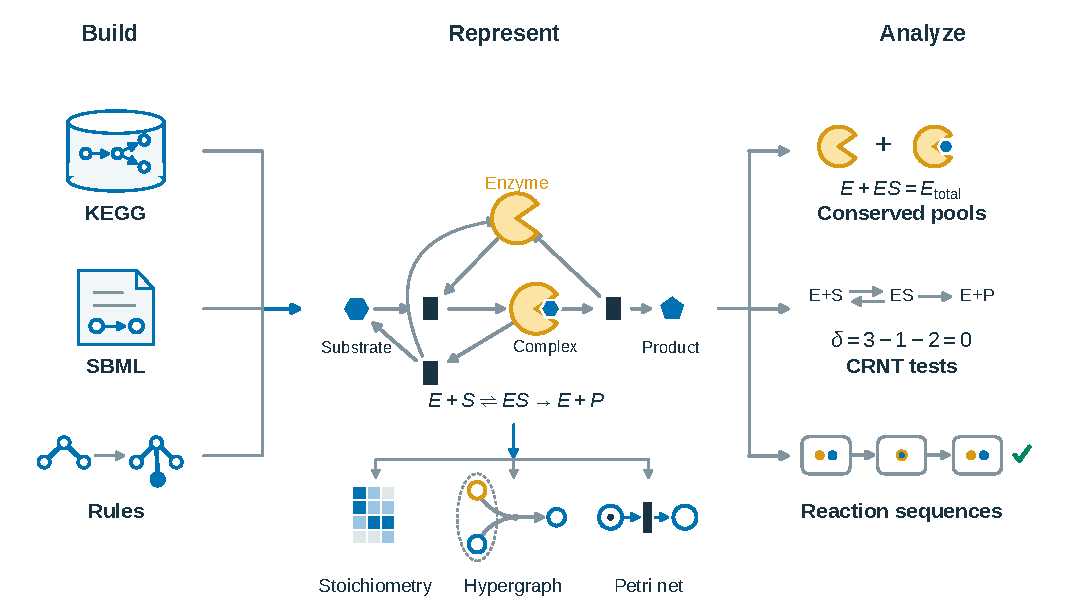
\includegraphics[width=\linewidth]{Figure/visual_abstract.pdf}
\caption{Overview of \synkitcrn workflows across construction, representation, and structural analysis. \textbf{Build:} Reaction networks imported from curated databases (\texttt{KEGG}), exchange files (\texttt{SBML}), or generated by rule expansion are mapped to a unified data structure. \textbf{Represent:} An illustrative enzyme mechanism ($E+S\rightleftharpoons ES\to E+P$) is converted into three complementary views: stoichiometric matrices, directed hypergraphs, and Petri nets, ensuring that multi-reactant requirements ($E$ and $S$) are captured as joint inputs. \textbf{Analyze:} These structural representations enable exact conservation analysis (identifying the conserved pool $E+ES$), chemical reaction network deficiency calculation ($\delta=0$), and discrete pathway realizability through verified firing sequences. Blue circles denote metabolites, orange circles denote enzymes, and dark bars represent reactions.}
\label{fig:synkit_architecture}
\end{figure}


For reaction $r$, reactant and product multisets have coefficients $s^-_{xr}$ and $s^+_{xr}$, defining separate reactant and product (pre/post) incidence matrices $\mathbf S^-=(s^-_{xr})$ and $\mathbf S^+=(s^+_{xr})$ alongside the net stoichiometry $\mathbf S=\mathbf S^+-\mathbf S^-$. Retaining participants present on both sides in both matrices preserves catalytic and cofactor requirements. Their net coefficients cancel in $\mathbf S$, but they still govern reaction enabling and define distinct reaction complexes (Fig.~\ref{fig:concepts}a,b). In Petri-net terms, such shared species form self-loops, and the net incidence matrix alone cannot determine whether transitions are enabled~\cite{murata1989petri}. Construction does not establish elemental balance automatically, so chemical interpretation requires suitable input equations and annotations. The conditions under which a reaction network represents genuine chemical transformations are themselves a subject of study~\cite{muller2022chemical}.

Reaction networks can be constructed from curated databases, generative chemistry, or standard model files. The \texttt{Query} module parses reaction equations from \texttt{KEGG}, \texttt{Construct} expands networks from chemical seeds using reaction rules, and \texttt{IO} imports models directly from \texttt{SBML}. During construction, reversible reactions can be partitioned into directed steps. Users can also choose whether to explicitly retain cofactors (such as ATP and NADH) and boundary species, which directly dictates the resulting conserved moieties, network deficiency, and discrete pathway realizability.

\subsection{Conserved moiety and stoichiometric analysis}
\label{sec:analysis}

The stoichiometric matrix $\mathbf S$ records the net change in every species for each reaction. For concentrations $c$ and reaction rates $v(c)$, the dynamics are written as $\dot c=\mathbf S v(c)$. A vector $y$ satisfying $y^T\mathbf S=0$ defines a conserved linear quantity $y^Tc$, because the reactions can redistribute the participating species without changing this weighted total. \synkitcrn computes a rational basis for the left nullspace of $\mathbf S$ and converts its vectors to primitive integer representatives. These vectors describe all rational conservation relations, but they need not be non-negative or identify the smallest conserved pools.

\begin{figure}[!htbp]
\centering
\begingroup
\definecolor{cInk}{HTML}{193342}
\definecolor{cBlue}{HTML}{0072B2}
\definecolor{cLBlue}{HTML}{9CC5E3}
\definecolor{cSpF}{HTML}{E4F0F8}
\definecolor{cOrange}{HTML}{D89915}
\definecolor{cOrF}{HTML}{FCE3A6}
\definecolor{cGreen}{HTML}{008564}
\definecolor{cMuted}{HTML}{81939D}
\definecolor{cPale}{HTML}{EEF3F6}
\definecolor{cRed}{HTML}{C8553D}
\definecolor{cRedF}{HTML}{F7DCD5}
\newcommand{\cB}{\scSans\fontsize{7}{8.4}\selectfont\color{cInk}}
\newcommand{\cS}{\scSans\fontsize{6.5}{7.8}\selectfont\color{cInk}}
\newcommand{\cT}{\scSans\fontsize{5.5}{6}\selectfont\color{cMuted}}
\tikzset{
  csyn/.style={font=\scSans,color=cInk,
               execute at begin picture={\MTversion*{synsans}}},
  cpl/.style={circle,draw=cBlue,fill=cSpF,line width=0.6pt,
              minimum size=5.0mm,inner sep=0pt,font=\cB},
  cplS/.style={cpl,fill=cLBlue},
  cplR/.style={cpl,draw=cRed,fill=cRedF},
  cplE/.style={cpl,draw=cOrange,fill=cOrF},
  ctr/.style={rectangle,fill=cInk,draw=none,minimum width=1.2mm,
              minimum height=4.4mm,inner sep=0pt},
  ctrG/.style={ctr,fill=cMuted!50},
  carc/.style={-{Stealth[length=1.7mm,width=1.4mm]},line width=0.7pt,
               draw=cMuted,shorten >=0.4pt,shorten <=0.4pt},
  carcE/.style={carc,draw=cOrange},
  carcT/.style={carc,draw=cBlue,line width=1.3pt},
  carcR/.style={carc,draw=cRed,line width=1.3pt},
  carcG/.style={carc,draw=cMuted!45},
  cwt/.style={font=\cS,inner sep=0.6pt,fill=white},
  crl/.style={font=\cS,inner sep=0.8pt},
  ctxt/.style={font=\cB,align=left,anchor=north west,inner sep=0pt},
  chd/.style={font=\scSans\fontsize{7.5}{9}\selectfont\bfseries\color{cInk},
              anchor=north west,inner sep=0pt},
  cmk/.style={rectangle,rounded corners=2pt,draw=cMuted,fill=white,
              line width=0.6pt,minimum width=1.10cm,minimum height=0.66cm,
              inner sep=0pt},
}
\newcommand{\cpanel}[3]{%
  \node[anchor=base west,inner sep=0pt,
        font=\scSans\fontsize{9}{9}\selectfont\bfseries\color{cInk}] (cp#2)
        at ($#1+(0,-0.28)$) {#2};
  \node[chd,anchor=base west] at ($(cp#2.base east)+(0.18,0)$) {#3};}

\newcommand{\toynet}[1]{%
  \node[cpl]  (#1A) at (0,0)      {$A$};
  \node[ctr]  (#1r1) at (0.75,0)  {};
  \node[cpl]  (#1B) at (1.5,0)    {$B$};
  \node[ctr]  (#1r2) at (2.25,0)  {};
  \node[cpl]  (#1C) at (3.0,0)    {$C$};
  \node[ctr]  (#1r4) at (3.75,0)  {};
  \node[cpl]  (#1D) at (4.5,0)    {$D$};
  \node[cplE] (#1E) at (2.25,0.95) {$E$};
  \node[ctr,rotate=90] (#1r3) at (1.5,-0.80) {};
  \draw[carc] (#1A) -- (#1r1) node[cwt,midway,above=0.5pt] {2};
  \draw[carc] (#1r1) -- (#1B);
  \draw[carc] (#1B) -- (#1r2);
  \draw[carc] (#1r2) -- (#1C);
  \draw[carc] (#1C) -- (#1r4);
  \draw[carc] (#1r4) -- (#1D);
  \draw[carcE] (#1E) to[bend right=28] (#1r2);
  \draw[carcE] (#1r2) to[bend right=28] (#1E);
  \draw[carc] (#1C) |- (#1r3);
  \draw[carc] (#1r3) -| (#1A) node[cwt,pos=0.78,left=0.5pt] {2};
  \node[crl,below=1.2pt] at (#1r1.south) {$r_1$};
  \node[crl,below=1.2pt] at (#1r2.south) {$r_2$};
  \node[crl] at ($(#1r3)+(0,-0.22)$) {$r_3$};
  \node[crl,below=1.2pt] at (#1r4.south) {$r_4$};
}

\def\cw{0.37}\def\rh{0.33}
\newcommand{\cmat}[4]{%
  \node[font=\cB,anchor=south] at ({#1+1.5*\cw},{#2+0.36}) {#3};
  \foreach \lab [count=\j from 0] in {r_1,r_2,r_3,r_4}
    \node[font=\cT] at ({#1+\j*\cw},{#2+0.26}) {$\lab$};
  \foreach \row [count=\i from 0] in {#4} {
    \foreach \v [count=\j from 0] in \row {
      \ifnum\v=0
        \node[fill=cPale,minimum width=0.34cm,minimum height=0.30cm,inner sep=0pt]
          at ({#1+\j*\cw},{#2-\i*\rh}) {};
      \else
        \ifnum\i=4
          \node[fill=cOrF,draw=cOrange,line width=0.5pt,minimum width=0.34cm,
            minimum height=0.30cm,inner sep=0pt,font=\cS]
            at ({#1+\j*\cw},{#2-\i*\rh}) {$\v$};
        \else\ifnum\numexpr\v*\csign\relax<0
          \node[fill=cBlue,minimum width=0.34cm,minimum height=0.30cm,inner sep=0pt,
            font=\cS,text=white] at ({#1+\j*\cw},{#2-\i*\rh}) {$\v$};
        \else
          \node[fill=cLBlue,minimum width=0.34cm,minimum height=0.30cm,inner sep=0pt,
            font=\cS] at ({#1+\j*\cw},{#2-\i*\rh}) {$\v$};
        \fi\fi
      \fi}}
}

\newcommand{\cmark}[7]{%
  \node[cmk] (#1) at #2 {};
  \foreach \n/\col [count=\k from 0] in {#3/cBlue,#4/cBlue,#5/cBlue,#6/cBlue,#7/cOrange} {
    \pgfmathsetmacro\sx{-0.42+\k*0.21}
    \ifnum\n>0 \fill[\col] ($(#1.center)+(\sx,0.07)$) circle (0.06); \fi
    \ifnum\n>1 \fill[\col] ($(#1.center)+(\sx,0.21)$) circle (0.06); \fi
  }
  \foreach \lab [count=\k from 0] in {A,B,C,D,E} {
    \pgfmathsetmacro\sx{-0.42+\k*0.21}
    \node[font=\cT] at ($(#1.center)+(\sx,-0.19)$) {$\lab$};}
}
\newcommand{\cyes}{\tikz[baseline=-0.6ex,-]{\draw[cGreen,line width=1.1pt,
  line cap=round,line join=round] (-0.085,0.0) -- (-0.02,-0.07) -- (0.10,0.08);}}
\newcommand{\cno}{\tikz[baseline=-0.6ex,-]{\draw[cRed,line width=1.1pt,line cap=round]
  (-0.07,-0.07) -- (0.07,0.07) (-0.07,0.07) -- (0.07,-0.07);}}

\begin{tikzpicture}[csyn]
\path[use as bounding box] (0,0) rectangle (16.40,-10.05);

\cpanel{(0.05,-0.05)}{a}{Reaction network}
\begin{scope}[shift={(0.45,-2.10)}]
  \toynet{a}
\end{scope}
\node[ctxt] at (0.30,-3.65) {%
  $r_1\colon 2A\to B$\qquad\ \ $r_2\colon B+E\to C+E$\\[1pt]
  $r_3\colon C\to 2A$\qquad\ \ $r_4\colon C\to D$};

\cpanel{(5.60,-0.05)}{b}{Incidence and net stoichiometry}
\def\my{-1.70}
\fill[cOrF!45,rounded corners=1.5pt] (5.78,{\my-4*\rh+0.21}) rectangle (11.35,{\my-4*\rh-0.21});
\foreach \s [count=\i from 0] in {A,B,C,D}
  \node[font=\cB,anchor=east] at (6.12,{\my-\i*\rh}) {$\s$};
\node[font=\cB,anchor=east,text=cOrange] at (6.12,{\my-4*\rh}) {$E$};
\def\csign{-1}\cmat{6.40}{\my}{$\mathbf S^-$}{{2,0,0,0},{0,1,0,0},{0,0,1,1},{0,0,0,0},{0,1,0,0}}
\def\csign{1}\cmat{8.20}{\my}{$\mathbf S^+$}{{0,0,2,0},{1,0,0,0},{0,1,0,0},{0,0,0,1},{0,1,0,0}}
\cmat{10.00}{\my}{$\mathbf S$}{{-2,0,2,0},{1,-1,0,0},{0,1,-1,-1},{0,0,0,1},{0,0,0,0}}
\node[font=\cB] at (8.57,-3.55) {$\mathbf S=\mathbf S^+-\mathbf S^-$};

\cpanel{(11.45,-0.05)}{c}{Semiflows}
\begin{scope}[shift={(11.85,-1.40)},x=0.86cm]
  \node[cplS] (pA) at (0,0)   {$A$};
  \node[ctr]  (p1) at (0.75,0) {};
  \node[cplS] (pB) at (1.5,0) {$B$};
  \node[ctr]  (p2) at (2.25,0) {};
  \node[cplS] (pC) at (3.0,0) {$C$};
  \node[ctr]  (p4) at (3.75,0) {};
  \node[cplS] (pD) at (4.5,0) {$D$};
  \node[cplE,double,double distance=0.8pt] (pE) at (2.25,0.80) {$E$};
  \draw[carc] (pA) -- (p1); \draw[carc] (p1) -- (pB);
  \draw[carc] (pB) -- (p2); \draw[carc] (p2) -- (pC);
  \draw[carc] (pC) -- (p4); \draw[carc] (p4) -- (pD);
  \draw[carcE] (pE) to[bend right=28] (p2);
  \draw[carcE] (p2) to[bend right=28] (pE);
  \foreach \n/\w in {pA/1,pB/2,pC/2,pD/2}
    \node[font=\cS,text=cBlue,below=1.0pt] at (\n.south) {$\times\w$};
\end{scope}
\node[ctxt] at (11.70,-2.15) {%
  P-semiflows $y^{\mathsf T}\mathbf S=0$, $y\ge0$:\\
  \textcolor{cBlue}{$y_1$: $A+2B+2C+2D$}\\
  \textcolor{cOrange}{$y_2$: $E$}};
\begin{scope}[shift={(11.85,-3.70)},x=0.86cm]
  \node[cpl] (tA) at (0,0)   {$A$};
  \node[ctr] (t1) at (0.75,0) {};
  \node[cpl] (tB) at (1.5,0) {$B$};
  \node[ctr] (t2) at (2.25,0) {};
  \node[cpl] (tC) at (3.0,0) {$C$};
  \node[ctrG] (t4) at (3.75,0) {};
  \node[cpl,draw=cMuted!50,fill=white,text=cMuted!70] (tD) at (4.5,0) {$D$};
  \node[ctr,rotate=90] (t3) at (1.5,-0.62) {};
  \draw[carcT] (tA) -- (t1); \draw[carcT] (t1) -- (tB);
  \draw[carcT] (tB) -- (t2); \draw[carcT] (t2) -- (tC);
  \draw[carcT] (tC) |- (t3); \draw[carcT] (t3) -| (tA);
  \draw[carcG] (tC) -- (t4); \draw[carcG] (t4) -- (tD);
  \node[crl,above=1.2pt] at (t1.north) {$r_1$};
  \node[crl,above=1.2pt] at (t2.north) {$r_2$};
  \node[crl] at ($(t3)+(0,0.22)$) {$r_3$};
  \node[crl,above=1.2pt,text=cMuted] at (t4.north) {$r_4$};
\end{scope}
\node[ctxt] at (11.70,-4.60) {%
  T-semiflow $\mathbf Sx=0$, $x\ge0$:\\
  \textcolor{cBlue}{$x=(1,1,1,0)$}};

\cpanel{(0.05,-5.45)}{d}{Siphons and traps}
\begin{scope}[shift={(0.45,-7.05)}]
  \node[cplR] (dA) at (0,0)      {$A$};
  \node[ctr]  (d1) at (0.75,0)   {};
  \node[cplR] (dB) at (1.5,0)    {$B$};
  \node[ctr]  (d2) at (2.25,0)   {};
  \node[cplR] (dC) at (3.0,0)    {$C$};
  \node[ctr]  (d4) at (3.75,0)   {};
  \node[cpl]  (dD) at (4.5,0)    {$D$};
  \node[cplE,double,double distance=0.8pt] (dE) at (2.25,0.95) {$E$};
  \node[ctr,rotate=90] (d3) at (1.5,-0.80) {};
  \draw[carc] (dA) -- (d1); \draw[carc] (d1) -- (dB);
  \draw[carc] (dB) -- (d2); \draw[carc] (d2) -- (dC);
  \draw[carcE] (dE) to[bend right=28] (d2);
  \draw[carcE] (d2) to[bend right=28] (dE);
  \draw[carc] (dC) |- (d3); \draw[carc] (d3) -| (dA);
  \draw[carcR] (dC) -- (d4); \draw[carcR] (d4) -- (dD);
  \node[crl,above=1.2pt,text=cRed] at (d4.north) {$r_4$};
\end{scope}
\node[font=\cS] (tab) at (2.70,-9.05) {%
  \setlength{\tabcolsep}{4pt}\begin{tabular}{@{}lccc@{}}
    \toprule
    minimal siphon & siphon & trap & covered\\
    \midrule
    \textcolor{cOrange}{$\{E\}$} & \cyes & \cyes & \cyes\\
    \textcolor{cRed}{$\{A,B,C\}$} & \cyes & \cno & \cno\\
    \bottomrule
  \end{tabular}};

\cpanel{(5.60,-5.45)}{e}{Pathway realizability of $f=(1,1,0,1)$}
\def\xa{7.45}\def\xb{9.05}\def\xc{10.65}\def\xd{12.25}
\def\xq{14.15}\def\xf{15.65}
\node[font=\cS,align=center] at (6.10,-6.30) {initial\\marking $m$};
\node[font=\cS,align=center] at (\xq,-6.30) {$D$ reachable\\(qualitative)};
\node[font=\cS,align=center] at (\xf,-6.30) {$f$ realizable\\(tokens)};
\def\ya{-7.05}
\node[font=\cB,anchor=west] at (5.80,\ya) {$2A{+}E$};
\cmark{m11}{(\xa,\ya)}{2}{0}{0}{0}{1}
\cmark{m12}{(\xb,\ya)}{0}{1}{0}{0}{1}
\cmark{m13}{(\xc,\ya)}{0}{0}{1}{0}{1}
\cmark{m14}{(\xd,\ya)}{0}{0}{0}{1}{1}
\draw[carc] (m11) -- (m12) node[crl,midway,above=1pt] {$r_1$};
\draw[carc] (m12) -- (m13) node[crl,midway,above=1pt] {$r_2$};
\draw[carc] (m13) -- (m14) node[crl,midway,above=1pt] {$r_4$};
\node[font=\cB] at (\xq,\ya) {\cyes};
\node[font=\cB] at (\xf,\ya) {\cyes};
\def\yb{-8.15}
\node[font=\cB,anchor=west] at (5.80,\yb) {$A{+}E$};
\cmark{m21}{(\xa,\yb)}{1}{0}{0}{0}{1}
\draw[carc,draw=cRed] (m21) -- ++(1.00,0) node[crl,pos=0.45,above=1pt] {$r_1$}
  node[font=\cB,anchor=west,inner sep=1pt,xshift=2pt] {\cno\ \ $m_A=1<2=s^-_{A r_1}$};
\node[font=\cB] at (\xq,\yb) {\cyes};
\node[font=\cB] at (\xf,\yb) {\cno};
\def\yc{-9.25}
\node[font=\cB,anchor=west] at (5.80,\yc) {$2A$};
\cmark{m31}{(\xa,\yc)}{2}{0}{0}{0}{0}
\cmark{m32}{(\xb,\yc)}{0}{1}{0}{0}{0}
\draw[carc] (m31) -- (m32) node[crl,midway,above=1pt] {$r_1$};
\draw[carc,draw=cRed] (m32) -- ++(1.00,0) node[crl,pos=0.45,above=1pt] {$r_2$}
  node[font=\cB,anchor=west,inner sep=1pt,xshift=2pt] {\cno\ \ $m_E=0<1=s^-_{E r_2}$};
\node[font=\cB] at (\xq,\yc) {\cno};
\node[font=\cB] at (\xf,\yc) {\cno};
\draw[line width=0.5pt,cMuted!50] (13.40,-6.00) -- (13.40,-9.75);
\end{tikzpicture}
\endgroup

\caption{Structural objects on one toy network, colored as in Fig.~\ref{fig:synkit_architecture}, with red marking blocked steps or uncovered sets. \textbf{(a)}~Petri net (circles: species, bars: reactions, arc labels: coefficients other than one). The enzyme $E$ is consumed and returned by $r_2$. \textbf{(b)}~Reactant, product, and net incidence matrices. The row of $E$ cancels in $\mathbf S$, so the net matrix alone does not show that $r_2$ requires $E$. \textbf{(c)}~P-semiflows (shaded, with weights) are conserved pools. The T-semiflow (heavy arcs) is a balanced reaction combination that fixes no firing order. \textbf{(d)}~Minimal siphons. $\{E\}$ contains a conserved pool and is covered, whereas $\{A,B,C\}$ drains through $r_4$ (heavy) and is uncovered. \textbf{(e)}~Firing from three initial markings (dots: tokens). From $A+E$, qualitative reachability reaches $D$ although no reaction is enabled. Inequalities give the failed condition $m_x\ge s^-_{xr}$.}
\label{fig:concepts}
\end{figure}

Minimal P-semiflows are computed separately by exact Farkas elimination~\cite{colom1991convex}. They are non-zero, non-negative integer vectors in the left kernel of $\mathbf S$ with inclusion-minimal supports, normalized by their greatest common divisor. Their supports identify minimal conserved pools of the represented network~\cite{famili2003leftnullspace}. A P-semiflow guarantees mathematical conservation, whereas assigning its support to a chemical moiety requires species annotations and biochemical interpretation.

T-semiflows satisfy $\mathbf Sx=0$ with $x\ge0$ and describe balanced combinations of reactions whose total net species change is zero. They are reaction-space relations, not conserved species pools (Fig.~\ref{fig:concepts}c). A T-semiflow fixes neither a firing order nor an initial marking, and it does not imply thermodynamic feasibility. All-positive left and right kernel vectors define conservativity and consistency, respectively. To determine positive-kernel feasibility, a linear program proposes a candidate vector that is accepted only after exact rational verification. Feasible networks are certified by an exact all-positive vector, infeasible networks by a rational separating vector, and unresolved solver outcomes remain undecided. Numerical kernel and Jacobian-pattern checks can also characterize approximate subspaces and qualitative matrix patterns, but because floating-point estimates do not isolate integer minimal supports, numerical rounding cannot substitute for exact conservation analysis.

\subsection{Deficiency analysis and multistationarity bounds}
\label{sec:crnt}

Complexes are distinct reactant or product multisets. With $n$ complexes, $\ell$ connected components of the complex graph (linkage classes), and stoichiometric rank $s$, deficiency is $\delta=n-\ell-s$.
A network is weakly reversible when every linkage class is strongly connected. \synkitcrn calculates ranks exactly over $\mathbb Q$ and reports the deficiency of the network and of each linkage class, weak reversibility, and the terminal strong linkage classes.

For positive mass-action rate constants, a weakly reversible deficiency-zero network has exactly one positive steady state in each positive stoichiometric compatibility class $(c_0+\operatorname{im}\mathbf S)\cap\mathbb R^{X}_{>0}$, and it is locally asymptotically stable relative to that class~\cite{horn1972general,feinberg1987deficiency}. A deficiency-zero network that is not weakly reversible has no positive steady state. The Deficiency One Theorem gives at most one positive steady state per positive stoichiometric compatibility class when each linkage-class deficiency is at most one, their sum equals $\delta$, and each linkage class has one terminal strong linkage class, while weak reversibility additionally ensures existence~\cite{feinberg1995existence}. Failure of these hypotheses leaves the corresponding theorem undecided. Introductions to this body of theory for biologists are available~\cite{gunawardena2003crnt}. Criteria that reach beyond deficiency, including injectivity~\cite{craciun2005injectivity}, concordance~\cite{shinar2012concordant}, and graph-theoretic multistationarity tests~\cite{mincheva2007graph1}, are not implemented here, and a network left undecided by the deficiency theorems is not thereby shown to be multistationary.

\subsection{Pathway realizability and siphon analysis}
\label{sec:petrinet}
\label{sec:pathway}

A siphon is a non-empty species set for which every reaction producing a member also consumes a member. Once empty, it cannot refill under Petri-net firing semantics. A trap has the dual property that every reaction consuming a member also produces a member, so a marked trap cannot become empty~\cite{murata1989petri}. \synkitcrn enumerates minimal siphons using implication propagation and closure minimization, within the branch-and-bound approach to structural enumeration~\cite{cordone2005enumeration}. Producing a selected species forces selection of a reactant. Selected and excluded species are propagated before branching. Each reported minimal set excludes its supersets from further search, and a maximal-closure deletion test verifies minimality. Traps use the dual incidence (Fig.~\ref{fig:concepts}d). This prunes many subsets but does not remove worst-case combinatorial growth.

The package checks whether every minimal siphon contains the support of a P-semiflow, and we call such a siphon covered. Under the boundedness and kinetic assumptions of the corresponding persistence result, this provides a sufficient persistence certificate for positive initial conditions~\cite{angeli2007persistence}. An uncovered siphon means the test is insufficient, and does not prove extinction or identify a unique nutrient supplementation strategy. The returned details expose these uncovered sets.

A marking $m$ specifies the non-negative integer inventory of each species. Reaction $r$ is enabled precisely when $m_x\ge s^-_{xr}$ for every species, and firing gives $m'=m+\mathbf S_{\cdot r}$. Qualitative reachability instead accumulates reachable species sets and ignores consumption and multiplicity. Given a requested flux $f\in\mathbb N_0^{|\mathscr R|}$, realizability search seeks an enabled sequence firing each reaction exactly $f_r$ times~\cite{andersen2023realisability}. A positive result includes a certificate consisting of an ordered reaction list that can be checked by updating the inventory after every step. An exhaustive negative result is \texttt{unrealizable}, while reaching a state or depth limit is \texttt{inconclusive}. Fig.~\ref{fig:concepts}e contrasts the two notions on one requested flux. Certificates establish firing in the specified discrete model only.

\subsection{Implementation and software comparison}
\label{sec:sbml}
\label{sec:usage}
\label{sec:comparison}

The software employs a hybrid architecture where users interact entirely through a high-level Python interface, while computationally intensive tasks are transparently dispatched to an optimized C++17 library. These native routines compute exact rational nullspaces, CRNT deficiency invariants, minimal semiflows, siphon enumeration, and discrete firing sequences. To eliminate floating-point rounding errors and ensure exact certificates, linear-algebraic and combinatorial routines use arbitrary-precision integer arithmetic via Boost.Multiprecision. For generative chemistry, \texttt{SynReactor} applies double-pushout graph transformations with implicit hydrogen counts. Its native C++ controller performs candidate construction, frontier updates, matching, rewriting, and reaction integration from seed molecules. Following the \texttt{M\O D} strategy framework~\cite{andersen2014strategies}, each rule application must use at least one newly generated molecule.

To ensure interoperability with the wider modeling community, \synkit provides native \texttt{SBML} Level~3 Core import and export. The parser preserves species identifiers, compartments, and exact stoichiometries across export and re-import, omitting kinetic rate laws and package extensions. Exported models provide the structural foundation for parameterization in kinetic simulators like \texttt{Tellurium} or constraint-based packages like \texttt{COBRApy}.

Through this design, \synkit occupies a distinct niche in the systems biology software ecosystem (Table~\ref{tab:software}). Established packages typically specialize in continuous kinetic simulation (\texttt{Tellurium}), flux-balance analysis (\texttt{COBRApy}), or algebraic deficiency testing (\texttt{CRNT4SBML}). While \texttt{crnpy} evaluates exact semiflows and \texttt{MolFoundry} solves rule-based hyperflows, \synkit unifies rule generation, deficiency, minimal siphons, and discrete firing certificates on a shared model. Downstream analyses can then build directly on exported \texttt{SBML} networks. Section~1 of the Supplementary Information and Listing~\ref{supp:lst:usage} provide complete implementation details and usage examples.

\begin{table}[!htbp]
\centering
\caption{Feature comparison of biochemical reaction-network software (\yes{} supported, \pmark{} partial or indirect as detailed in footnotes, \no{} not supported). Capabilities are determined from official documentation and source code. \texttt{CRNT4SBML} is experimentally evaluated on shared benchmark networks (Table~\ref{tab:reference}); formose generation is compared with \texttt{M\O D} and \texttt{MolFoundry}, and fixed-route realizability with \texttt{MolFoundry} (Section~\ref{sec:usecase_expand}). The \synkit column describes its chemical reaction network (CRN) submodule.}
\label{tab:software}
\footnotesize
\setlength{\tabcolsep}{4pt}
\renewcommand{\arraystretch}{1.06}
\begin{tabular*}{\linewidth}{@{\extracolsep{\fill}}l cccccccc@{}}
\toprule
 & \rot{\texttt{SynKit} (this work)}
 & \rot{\texttt{CRNT4SBML}~\cite{reyes2020crnt4sbml}}
 & \rot{\texttt{CoNtRol}~\cite{donnell2014control}}
 & \rot{\texttt{crnpy}~\cite{tonello2016crnpy}}
 & \rot{\texttt{COBRApy}~\cite{ebrahim2013cobrapy}}
 & \rot{\texttt{M\O D}~\cite{andersen2016mod}}
 & \rot{\texttt{MolFoundry}~\cite{friedrichs2026molfoundry}}
 & \rot{\texttt{Tellurium}~\cite{choi2018tellurium,welsh2023libroadrunner}} \\
\midrule
\multicolumn{9}{@{}l}{\emph{Network construction and exchange}}\\
\quad \texttt{KEGG} pathway import                     & \yes & \no  & \no  & \no  & \no  & \no  & \no  & \no  \\
\quad \texttt{SBML} import                             & \pmark\textsuperscript{a} & \yes & \no & \yes & \yes & \no & \no & \yes \\
\quad \texttt{SBML} export                             & \pmark\textsuperscript{a} & \no  & \no  & \yes & \yes & \no  & \yes & \yes \\
\quad Rule-based network generation           & \yes & \no  & \no  & \no  & \no  & \yes & \yes & \no  \\
\addlinespace[3pt]
\multicolumn{9}{@{}l}{\emph{Structural analysis}}\\
\quad Deficiency and weak reversibility (CRNT) & \yes & \yes & \yes & \yes & \no & \no & \no & \no \\
\quad Conservation laws (left-nullspace basis)& \yes & \yes & \no  & \yes & \no  & \no  & \no  & \yes \\
\quad Minimal semi-positive conservation laws & \yes & \no  & \no  & \yes & \no  & \no  & \no  & \no  \\
\quad Elementary flux modes or T-semiflows    & \yes & \no  & \no  & \yes & \no  & \no  & \no  & \no  \\
\quad Minimal siphons and traps               & \yes & \no  & \pmark\textsuperscript{b} & \no & \no & \no & \no & \no \\
\addlinespace[3pt]
\multicolumn{9}{@{}l}{\emph{Dynamics and pathway feasibility}}\\
\quad Multistationarity analysis             & \no  & \yes & \yes & \pmark\textsuperscript{c} & \no & \no & \no & \no \\
\quad Pathway realizability (firing sequence)& \yes & \no  & \no  & \no  & \no  & \pmark\textsuperscript{d} & \yes\textsuperscript{f} & \no \\
\quad Constraint-based modeling (e.g., FBA)  & \no  & \no  & \no  & \no  & \yes & \no  & \pmark\textsuperscript{f} & \no  \\
\quad Kinetic simulation                      & \no  & \pmark\textsuperscript{e} & \no & \no & \no & \no & \yes\textsuperscript{g} & \yes \\
\bottomrule
\end{tabular*}

\vspace{2pt}
\begin{minipage}{\linewidth}\footnotesize
\begin{tabular}{@{}r@{~}p{0.95\linewidth}@{}}
\textsuperscript{a} & \texttt{SBML} Level~3 Version~2 Core reaction structure only, with kinetic laws and rules not handled. \\
\textsuperscript{b} & Siphons underlie persistence tests, but minimal-siphon enumeration is not exposed as an output. \\
\textsuperscript{c} & \texttt{crnpy} supplies Gr{\"o}bner-basis, elementary-mode, and ACR machinery rather than bistability search. \\
\textsuperscript{d} & \texttt{M\O D} evaluates integer hyperflows rather than discrete firing certificates over a finite marking. \\
\textsuperscript{e} & ODE simulation is provided in support of \texttt{CRNT4SBML}'s bistability analysis. \\
\textsuperscript{f} & \texttt{MolFoundry} solves integer hyperflows over derivation graphs (Gurobi or SMT) for firing orders. \\
\textsuperscript{g} & Rule-based stochastic simulation with on-demand network expansion. \\
\end{tabular}
\end{minipage}
\end{table}

\subsection{Validation and benchmark design}
\label{sec:validation_design}

We validate the toolkit through analytical benchmarks, runtime scaling experiments, and biochemical case studies. First, structural correctness is evaluated across twelve reference networks, including enzyme mechanisms, multisite phosphorylation cycles~\cite{wang2008multisite}, the bistable Edelstein switch~\cite{edelstein1970biochemical}, and the Shinar--Feinberg robustness motif~\cite{shinar2010structural}, with shared CRNT invariants independently confirmed by \texttt{CRNT4SBML}. Second, computational scaling for exact siphon and conserved-pool enumeration is profiled across synthetic topologies to establish practical tractability limits. Third, structural \texttt{SBML} exchange and deficiency preservation are evaluated across eleven curated \texttt{BioModels} entries spanning up to 504 species and 827 directed reactions.

Finally, two mechanistic case studies demonstrate how structural representation choices dictate pathway feasibility from finite metabolite pools. In \texttt{KEGG} glycolysis, we assess how retaining catalytic polyphosphate and closing adenine/nicotinamide cofactor cycles govern discrete pathway execution. In rule-generated formose chemistry, we contrast qualitative hypergraph reachability with stoichiometric realizability under finite precursor budgets. Each feasible pathway is confirmed by an ordered reaction sequence from available precursors, while infeasibility is proved through exhaustive search.

\section{Results and discussion}
\label{sec:usecase}

\subsection{Reference-network validation and comparison with \texttt{CRNT4SBML}}
\label{sec:results_validation}

All twelve reference networks match their analytical and algebraic ground-truth values (Table~\ref{tab:reference}; sources and validation objectives detailed in Table~\ref{supp:tab:si_validation_sources}). The benchmark suite spans classic enzyme kinetics (Michaelis--Menten and its reversible counterpart), multisite phosphorylation cycles~\cite{wang2008multisite}, the bistable Edelstein switch~\cite{edelstein1970biochemical}, and the Shinar--Feinberg robustness motif~\cite{shinar2010structural}. In addition, constructed diagnostic cases verify boundary conditions: disconnected reversible pairs confirm that independent conserved pools are correctly isolated without conflating disjoint subnetworks, while the open reactor ($0 \to A \to B \to 0$) tests exact handling of inflow and outflow through the zero complex.

\begin{table}[!htbp]
\centering
\caption{Structural invariants of the twelve reference networks: species, directed reactions, complexes ($n$), linkage classes ($\ell$), stoichiometric rank ($s$), deficiency ($\delta$), conservation dimension (laws), and weak reversibility (WR). Every network matches its analytical and algebraic ground truth, and \texttt{CRNT4SBML} reproduces all eight shared structural quantities.}
\label{tab:reference}
\footnotesize
\begin{tabular*}{\linewidth}{@{\extracolsep{\fill}}l cccccccc@{}}
\toprule
Network & Species & Reactions & $n$ & $\ell$ & $s$ & $\delta$ & Laws & WR \\
\midrule
% BEGIN GENERATED: reference-networks
% Generated by analysis_overview.py from crn-validation.json.
Reversible isomerization & 2 & 2 & 2 & 1 & 1 & 0 & 1 & yes \\
Irreversible isomerization & 2 & 1 & 2 & 1 & 1 & 0 & 1 & no \\
Isomerization cycle & 3 & 3 & 3 & 1 & 2 & 0 & 1 & yes \\
Disconnected reversible pairs & 6 & 6 & 6 & 3 & 3 & 0 & 3 & yes \\
Pairs with stoichiometry & 6 & 6 & 6 & 3 & 3 & 0 & 3 & yes \\
Michaelis--Menten & 4 & 3 & 3 & 1 & 2 & 0 & 2 & no \\
Reversible Michaelis--Menten & 4 & 4 & 3 & 1 & 2 & 0 & 2 & yes \\
Edelstein switch & 3 & 6 & 5 & 2 & 2 & 1 & 1 & yes \\
Phosphorylation: one site & 6 & 6 & 6 & 2 & 3 & 1 & 3 & no \\
Phosphorylation: two sites & 9 & 12 & 10 & 2 & 6 & 2 & 3 & no \\
Shinar--Feinberg motif & 2 & 2 & 4 & 2 & 1 & 1 & 1 & no \\
Open reactor & 2 & 3 & 3 & 1 & 2 & 0 & 0 & yes \\
% END GENERATED: reference-networks
\bottomrule
\end{tabular*}
\end{table}

To benchmark structural interoperability, \texttt{CRNT4SBML}~0.0.15 independently parsed all twelve exported \texttt{SBML} models. Across all twelve benchmarks, both tools yielded identical results for all eight shared structural quantities (Table~\ref{tab:reference}), confirming topological consistency across independent implementations. Furthermore, standard floating-point nullspace methods produce numerical residuals on all closed networks, where naive scaling and rounding fail to recover valid integer conservation vectors on three of the twelve models (Table~\ref{supp:tab:numerical_audit}). In contrast, \synkit's exact rational arithmetic guarantees that the conservation identity $y^T \mathbf{S} = 0$ holds strictly across all networks without numerical rounding error.

\subsection{Computational cost of exact structural enumeration}
\label{sec:results_scaling}

Enumerating minimal siphons (Fig.~\ref{fig:concepts}d) and exact conserved pools (Fig.~\ref{fig:concepts}c) identifies extinction-prone species sets and mass conservation laws, but naive search scales exponentially with $2^N - 1$ candidate subsets. To prevent combinatorial explosion, implication pruning propagates stoichiometric constraints along active reactions during search (Fig.~\ref{fig:scaling}a). In reversible chains, selecting an initial species forces each adjacent neighbor, isolating the entire chain as the unique minimal siphon without evaluating spurious sub-combinations. Across five repeats per size, pruned search returns identical siphon sets with a \ReviewRatioLarge-fold speedup at 21 species (\ReviewClosureMilliseconds~ms versus \ReviewExhaustiveMilliseconds~ms for exhaustive search, Fig.~\ref{fig:scaling}b).

\begin{figure}[!htbp]
\centering
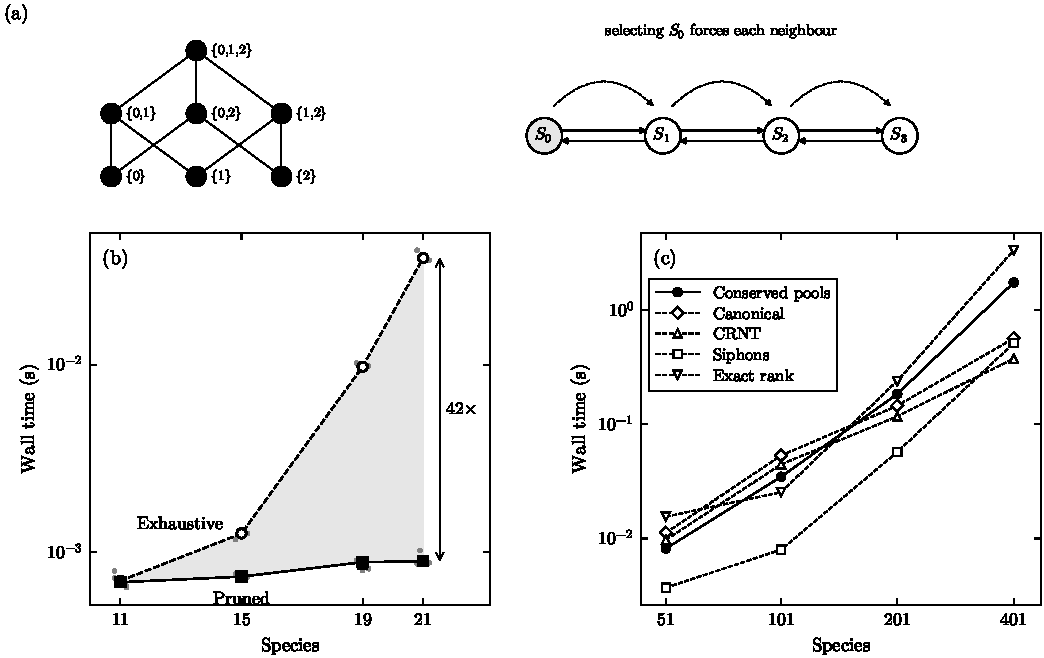
\includegraphics[width=\linewidth]{Figure/scaling.pdf}
\caption{Search algorithms and runtime scaling on reversible-chain networks. \textbf{(a)}~Schematic of exhaustive power-set search versus implication pruning, where selecting $S_0$ forces all chain species into the minimal siphon. \textbf{(b)}~Minimal-siphon runtimes across five repeats per size (points: individual runs, markers: medians and IQRs, bracket: speedup ratio at 21 species). \textbf{(c)}~Wall times for five structural analyses across chains up to 401 species.}
\label{fig:scaling}
\end{figure}

The broader benchmark suite evaluates scalability across directed chains, reversible chains, and random sparse bimolecular networks (Fig.~\ref{supp:fig:performance_diagnostics}). All 60 requested configurations complete without numerical failure. On the 401-species reversible chain, minimal siphons (Fig.~\ref{fig:concepts}d) take \ReviewReversibleSiphonSeconds~s, canonicalization \ReviewReversibleCanonicalSeconds~s, exact conserved pools (Fig.~\ref{fig:concepts}c) \ReviewReversibleMoietySeconds~s, and standalone exact rank \ReviewReversibleRankSeconds~s (Fig.~\ref{fig:scaling}c). The random networks with 49, 99, 197, and 395 species contain 331, 272, 47, and 87 minimal siphons, completing siphon and conserved-pool enumeration in \ReviewRandomSiphonSeconds~s and \ReviewRandomMoietySeconds~s at 395 species. Stoichiometric implication pruning and rational nullspace methods thus keep exact structural enumeration computationally practical on networks with hundreds of species.

\subsection{Structural \texttt{SBML} round-trip validation in \texttt{BioModels}}
\label{sec:results_biomodels}

To test real-world structural interoperability and scalability, we evaluated eleven curated \texttt{BioModels}~\cite{maliksheriff2020biomodels} entries spanning diverse sizes, including ten reaction networks and one qualitative network control (\texttt{SBML-qual}). All ten reaction-bearing models successfully round-trip through \synkit's \texttt{SBML} parser and exporter without loss of stoichiometry, and their deficiency values match the analytical identities (details in Table~\ref{supp:tab:biomodels_models}). Even on the largest model (\texttt{BIOMD0000000255}, with 504 species and 827 directed reactions), \synkit identifies 75 minimal siphons in \ReviewBioModelSiphonSeconds~s and 17 exact conserved pools in \ReviewBioModelMoietySeconds~s (Fig.~\ref{fig:evidence_overview}a). Testing siphon coverage by conserved pools evaluates whether species are structurally protected from extinction. In \texttt{BIOMD0000000255} and the 100-species model \texttt{BIOMD0000000019} (20 siphons, 19 pools), at least one minimal siphon lacks a supporting conserved pool, indicating that these cascades contain components that can drain to extinction unless sustained by continuous replenishment. The qualitative control \texttt{BIOMD0000000562} is correctly identified as reaction-free for Core structural analysis.

\begin{figure}[!htbp]
    \centering
    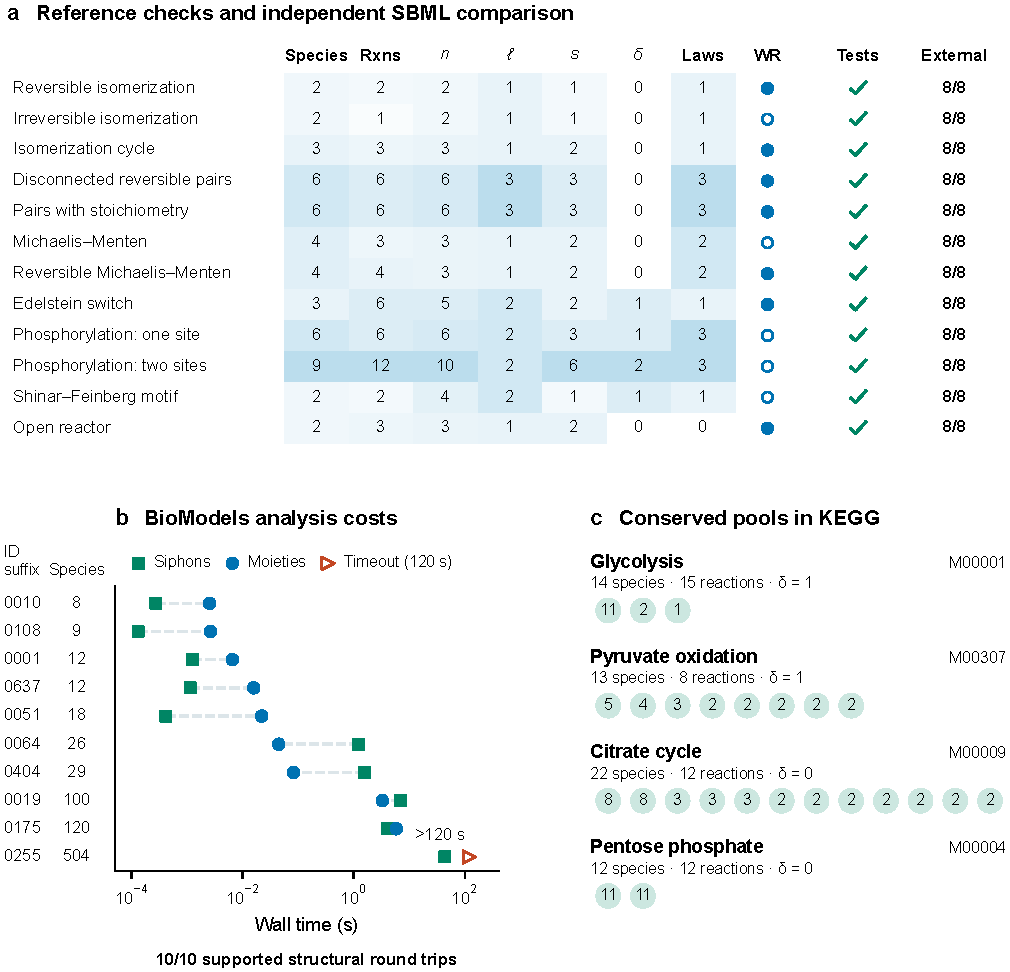
\includegraphics[width=\linewidth]{Figure/analysis_overview.pdf}
    \caption{Enumeration runtimes in \texttt{BioModels} and conserved pools in \texttt{KEGG} modules. \textbf{(a)}~Wall time for completed minimal-siphon and exact conserved-pool enumeration in ten reaction-bearing \texttt{BioModels} models. All ten models complete both enumerations. \textbf{(b)}~Minimal non-negative conserved pools in four reduced \texttt{KEGG} modules. Each dot is one pool placed at its number of species, pools of equal size are stacked, and the dotted line spans the module species, ending at the module size.}
    \label{fig:evidence_overview}
\end{figure}

\subsection{Conservation and cofactor requirements in glycolysis}
\label{sec:results_kegg}

Four \texttt{KEGG}~\cite{kanehisa2025kegg} pathway modules illustrate structural conservation across metabolic subsystems: glycolysis (\texttt{M00001}), pyruvate oxidation (\texttt{M00307}), the citrate cycle (\texttt{M00009}), and the pentose phosphate pathway (\texttt{M00004}). Their conserved-pool supports appear in Fig.~\ref{fig:evidence_overview}b. In the reduced citrate-cycle network, minimal non-negative conservation vectors automatically isolate key metabolic moiety pools, recovering nucleotide pairs, a quinone pair, a ferredoxin pair, coenzyme~A, and a lipoyl cofactor pool without manual annotation.

The reduced glycolysis model contains 14 species and 15 directed reactions ($n=16$, $\ell=4$, rank $s=11$, and deficiency $\delta=1$). Its primary conserved moiety spans eleven carbohydrate intermediates, assigning weight two to hexoses and one to trioses (Fig.~\ref{fig:glycolysis}), capturing exact three-carbon backbone conservation across aldolase cleavage. Glucose and oxidized ferredoxin form uncovered singleton siphons requiring replenishment, whereas polyphosphate forms a covered siphon because glucokinase retains the polymer on both sides.

From a single initial glucose molecule, the prescribed glycolytic flux yields a certified 15-step pathway realization terminating in two pyruvates, exploring 30 intermediate markings. Aldolase cleavage generates two triose equivalents that feed the repeated lower payoff phase. Step-by-step certificate replay confirms intermediate availability at every enzyme step and verifies exact invariance of the weighted three-carbon backbone pool ($2\times\text{hexoses} + 1\times\text{trioses} = 2$). Attempting to execute the lower payoff phase from glucose alone fails because the preparatory intermediates have not yet formed.

\begin{figure}[!htbp]
    \centering
    % ---------------------------------------------------------------------------
% glycolysis.tex --- KEGG M00001 end to end: topology, exact structure, the
% returned firing certificate, and every recorded token marking.
%
% Source fragment: loaded directly by main.tex.
%
% Every number comes from Figure/glycolysis_analysis.tex, regenerated by
% Figure/glycolysis_analysis.py from the cached module.
%
% Top panels show the reduced pathway and exact structural diagnostics.
% The full-width lower panel is generated from the complete recorded trajectory.
% ---------------------------------------------------------------------------
% Resolve the shared style and generated analysis macros from the manuscript
% root.
\IfFileExists{synstyle.tex}{\input{synstyle}}{%
  \IfFileExists{Figure/synstyle.tex}{% ---------------------------------------------------------------------------
% synstyle.tex --- shared look for every TikZ figure of the SynKit CRN paper.
%
% Input it from a figure file:
%     \IfFileExists{synstyle.tex}{\input{synstyle}}{% ---------------------------------------------------------------------------
% synstyle.tex --- shared look for every TikZ figure of the SynKit CRN paper.
%
% Input it from a figure file:
%     \IfFileExists{synstyle.tex}{\input{synstyle}}{\input{Figure/synstyle}}
% so that the figure compiles both from Figure/ and from the paper root.
%
% The visual vocabulary follows ../../../../Style/style.tex: the
% colour-blind-safe Okabe--Ito accents, quiet neutral rules and wash, circular
% panel badges, and a compact technical type scale are shared by the companion
% papers.  Semantic aliases below keep the CRN meaning explicit.
%
% DESIGN CONTRACT -----------------------------------------------------------
% 1. Geometry.  Every figure is laid out on a canvas exactly \scW wide (the
%    sn-jnl text width, 372 pt) and is included unscaled, so one point of type
%    is the same physical size in all five figures.  Open each picture with
%    \scCanvas{<height in cm>} to pin the bounding box.
% 2. Colour is semantic, never decorative.  Four roles only:
%       scAccent (green)       structure, the normal/expected path
%       scMark   (orange)      catalyst, certificate, or highlight
%       scAlert  (vermillion)  failure, violation, or uncovered set
%       scRef    (blue)        secondary or reference series
%    A panel gets at most one accent.  Titles are always ink; panel identity
%    is also encoded by a letter inside a circular badge, not by colour alone.
% 3. Type scale.  Three sizes, no others, and nothing below 6 pt:
%       \scTitle (7 pt bold)  panel titles
%       \scBody  (6.5 pt)     labels, values, in-figure prose
%       \scSmall (6 pt)       units, footnotes, dense graph labels
% ---------------------------------------------------------------------------
% Load guard.  The paper inputs every figure source inline, so this file is
% reached once per figure; without the guard the second \newlength below
% would abort the run.
\ifdefined\SynKitStyleLoaded\endinput\fi
\newcommand{\SynKitStyleLoaded}{}

% Load in the document preamble. XeLaTeX/LuaLaTeX and an installed Arial
% family are required; fontspec reports an error instead of substituting.
\RequirePackage[no-math]{fontspec}
\newfontfamily\scArial{Arial}[NFSSFamily=scArial,Ligatures=TeX]
% Keep manuscript mathematics unchanged; select Arial letters and numerals
% only inside figures. TeX supplies specialist mathematical symbols.
\RequirePackage[subdued,italic]{mathastext}
\MTDeclareVersion{synarial}{TU}{scArial}{m}{n}
\SetMathAlphabet{\Mathsf}{synarial}{TU}{scArial}{m}{n}
\SetMathAlphabet{\Mathtt}{synarial}{TU}{scArial}{m}{n}

\usetikzlibrary{positioning,calc,fit,backgrounds,arrows.meta,shapes.geometric,
                shapes.misc,decorations.pathreplacing,patterns,math}

% --- canvas ---------------------------------------------------------------
% 372 pt text width minus the 1 pt standalone border on each side.
\newlength{\scW}\setlength{\scW}{13.0326cm}
\providecommand{\scWnum}{13.0326}
% \scCanvas{<height>} pins the picture to the full text width, y running down
% from 0, so every figure shares one coordinate convention.  It *sets* the
% bounding box rather than contributing to it, so the emitted page is exactly
% the text width and every figure is included at 1:1 -- otherwise a stray
% invisible extent (pgfplots reserves a little around an axis) rescales one
% figure relative to the others and the same \scSmall prints at two sizes.
% Anything drawn outside the canvas is therefore cropped: keep content inside,
% and check with
%     \providecommand{\scCanvas}[1]{\path[draw=red] (0,0) rectangle (\scWnum,-#1);}
\providecommand{\scCanvas}[1]{%
  \path[use as bounding box] (0,0) rectangle (\scWnum,-#1);}

% --- palette --------------------------------------------------------------
% Canonical companion-paper values (../../../../Style/style.tex).
\definecolor{npgOrange}{HTML}{E69F00}
\definecolor{npgSky}{HTML}{56B4E9}
\definecolor{npgGreen}{HTML}{009E73}
\definecolor{npgYellow}{HTML}{F0E442}
\definecolor{npgBlue}{HTML}{0072B2}
\definecolor{npgVermillion}{HTML}{E64B35}
\definecolor{npgPurple}{HTML}{CC79A7}
\definecolor{figInk}{HTML}{1A1A1A}
\definecolor{figMuted}{HTML}{666666}
\definecolor{figHair}{HTML}{D9D9D9}
\definecolor{figWash}{HTML}{F7F7F7}

\colorlet{scInk}{figInk}              % primary text
\colorlet{scInkM}{figMuted}           % secondary text
\colorlet{scPaper}{figWash}           % quiet cards and note strips
\colorlet{scSpF}{npgSky!12}           % species fill
\colorlet{scSpE}{npgBlue}             % species edge
\colorlet{scRxF}{npgOrange!12}        % reaction fill
\colorlet{scRxE}{npgOrange!88!black}  % reaction edge
\colorlet{scReac}{npgBlue!78!black}   % reactant edge
\colorlet{scProd}{npgGreen!82!black}  % product edge
\colorlet{scHiF}{npgOrange!13}        % highlight fill
\colorlet{scHiE}{npgOrange!82!black}  % highlight edge
% Stage / accent tints.  stDE remains available for the fifth plot series.
\colorlet{stAF}{npgGreen!9}\colorlet{stAE}{npgGreen}
\colorlet{stBF}{npgOrange!11}\colorlet{stBE}{npgOrange}
\colorlet{stCF}{npgBlue!9}\colorlet{stCE}{npgBlue}
\colorlet{stDF}{npgPurple!10}\colorlet{stDE}{npgPurple!85!black}
\colorlet{stEF}{npgVermillion!9}\colorlet{stEE}{npgVermillion}

% Semantic aliases.  Figures should speak in these, not in stAE/stBE/...
\colorlet{scAccent}{stAE}\colorlet{scAccentF}{stAF}   % structure / normal
\colorlet{scMark}{stBE}\colorlet{scMarkF}{stBF}       % highlight / certificate
\colorlet{scRef}{stCE}\colorlet{scRefF}{stCF}         % secondary series
\colorlet{scAlert}{stEE}\colorlet{scAlertF}{stEF}     % failure / violation
\colorlet{scRule}{figHair}                            % card and axis hairlines
\colorlet{scRuleL}{figHair!55}                        % grid, dividers

% --- text styles ----------------------------------------------------------
% Three sizes, fixed in points so they do not drift with the document class.
% Arial is shared by labels, headings, panel badges, and chemistry labels.
\providecommand{\scTitle}{\scArial\fontsize{7}{8.4}\selectfont\bfseries\color{scInk}}
\providecommand{\scBody}{\scArial\fontsize{6.5}{7.8}\selectfont\color{scInkM}}
\providecommand{\scSmall}{\scArial\fontsize{6}{7.2}\selectfont\color{scInkM}}
\providecommand{\scSub}[1]{{\scSmall\itshape #1}}
\providecommand{\scPanel}[1]{{\scTitle(#1)}}
% Numerals that carry a result: ink, not colour, so the eye reads the value.
\providecommand{\scNum}{\scArial\fontsize{10}{11}\selectfont\bfseries\color{scInk}}

% --- shared TikZ styles ---------------------------------------------------
\tikzset{
  % text never hyphenates inside a figure
  every node/.append style={execute at begin node={%
      \hyphenpenalty=10000 \exhyphenpenalty=10000 \hbadness=10000 }},
  syn/.style={font=\scArial,color=scInk,
              execute at begin picture={\MTversion*{synarial}},
              >={Stealth[round,length=2.4mm,width=1.9mm]}},
  % containers ------------------------------------------------------------
  % One card chrome for the whole paper: white, 3 pt radius, one hairline.
  panel/.style={rounded corners=2.5pt,fill=none,draw=scRule,line width=0.45pt},
  card/.style={rounded corners=2.2pt,fill=scPaper,draw=scRule,line width=0.45pt,
               inner sep=5pt,align=left,anchor=north west},
  % a quiet strip for a panel's closing fact
  note/.style={rounded corners=2.5pt,fill=scPaper,draw=scRuleL,line width=0.4pt,
               inner xsep=6pt,inner ysep=3.5pt,align=left,font=\scSmall},
  % small labelled value pill
  chip/.style={rounded corners=2pt,fill=scPaper,draw=scRule,line width=0.4pt,
               inner xsep=4pt,inner ysep=2pt,font=\scSmall},
  % Circular letter badge: the same accessible panel marker used in Style/*.
  hbullet/.style={circle,fill=scInk,text=white,draw=none,
                  font=\scArial\fontsize{6}{6}\selectfont\bfseries,
                  minimum size=4.2mm,inner sep=0pt},
  ctag/.style={font=\scTitle,anchor=north west,text=scInk},
  % CRN primitives --------------------------------------------------------
  species/.style={rounded rectangle,fill=scSpF,draw=scSpE,line width=0.45pt,
                  inner xsep=2.4pt,inner ysep=1.6pt,font=\scSmall,
                  text=scInk,minimum height=3.6mm},
  cofactor/.style={species,fill=scRefF,draw=scRef},
  catalyst/.style={species,fill=scHiF,draw=scHiE},
  rxn/.style={rectangle,fill=scRxF,draw=scRxE,line width=0.45pt,
              inner sep=1.2pt,font=\scSmall,text=scInk,
              minimum width=3.0mm,minimum height=3.0mm},
  place/.style={circle,fill=scSpF,draw=scSpE,line width=0.45pt,
                minimum size=4.0mm,inner sep=0pt},
  trans/.style={rectangle,fill=scRxE,draw=scRxE,minimum width=1.1mm,
                minimum height=3.6mm,inner sep=0pt},
  token/.style={circle,fill=scInk,minimum size=1.1mm,inner sep=0pt},
  % edges -----------------------------------------------------------------
  reac/.style={->,line width=0.5pt,draw=scReac,shorten >=0.8pt,shorten <=0.8pt},
  prod/.style={->,line width=0.5pt,draw=scProd,shorten >=0.8pt,shorten <=0.8pt},
  cat/.style={->,line width=0.5pt,draw=scHiE,shorten >=0.8pt,shorten <=0.8pt},
  flow/.style={-{Stealth[round,length=2.2mm,width=1.8mm]},line width=1.1pt,
               draw=scInkM!45},
  flab/.style={font=\scSmall,text=scInkM,inner sep=2pt},
  stoi/.style={font=\scSmall,text=scInkM,inner sep=0.8pt},
  % verdict marks: shape carries the meaning, colour only reinforces it
  vpass/.style={circle,fill=scAccentF,draw=scAccent,text=scAccent,
                font=\fontsize{6}{6}\selectfont\bfseries,
                minimum size=3.2mm,inner sep=0pt},
  vfail/.style={circle,fill=scAlertF,draw=scAlert,text=scAlert,
                font=\fontsize{6}{6}\selectfont\bfseries,
                minimum size=3.2mm,inner sep=0pt},
  callout/.style={font=\scSmall,text=scInkM,align=left},
}

% \scHead[<badge colour>]{<anchor coord>}{<letter>}{<title>}{<subtitle or empty>}
% One header treatment for every panel in the paper.
\providecommand{\scHead}[5][scInk]{%
  \node[hbullet,fill=#1,anchor=north west] (scbadge#3) at ($#2+(0,-0.015)$)
    {\MakeUppercase{#3}};
  \node[ctag,anchor=west] at ($(scbadge#3.east)+(0.14,0)$) {#4};
  \ifx\relax#5\relax\else
    \node[anchor=north west,font=\scSmall,text=scInkM]
      at ($#2+(0.56,-0.245)$) {#5};
  \fi}

% --- shared pgfplots look (only if the figure loaded pgfplots) ------------
\ifdefined\pgfplotsset
  \pgfplotsset{compat=1.18}
  \pgfplotsset{
    synaxis/.style={
      scale only axis,
      tick align=outside, tick pos=left,
      axis line style={draw=scInkM!55,line width=0.4pt},
      % One grid, on the value axis only.  No minor grid: at these sizes it
      % turns the plot frame into a grey wash.
      ymajorgrids=true, xmajorgrids=false,
      major grid style={draw=scRuleL,line width=0.3pt},
      major tick length=1.6pt,
      label style={font=\scBody,color=scInk},
      tick label style={font=\scSmall,color=scInkM},
      legend style={font=\scSmall,draw=none,fill=none,inner sep=1pt,
                    row sep=0.4pt,legend columns=1},
      legend cell align=left,
      every axis plot/.append style={line width=0.7pt,mark size=1.2pt},
    },
  }
\fi
}
% so that the figure compiles both from Figure/ and from the paper root.
%
% The visual vocabulary follows ../../../../Style/style.tex: the
% colour-blind-safe Okabe--Ito accents, quiet neutral rules and wash, circular
% panel badges, and a compact technical type scale are shared by the companion
% papers.  Semantic aliases below keep the CRN meaning explicit.
%
% DESIGN CONTRACT -----------------------------------------------------------
% 1. Geometry.  Every figure is laid out on a canvas exactly \scW wide (the
%    sn-jnl text width, 372 pt) and is included unscaled, so one point of type
%    is the same physical size in all five figures.  Open each picture with
%    \scCanvas{<height in cm>} to pin the bounding box.
% 2. Colour is semantic, never decorative.  Four roles only:
%       scAccent (green)       structure, the normal/expected path
%       scMark   (orange)      catalyst, certificate, or highlight
%       scAlert  (vermillion)  failure, violation, or uncovered set
%       scRef    (blue)        secondary or reference series
%    A panel gets at most one accent.  Titles are always ink; panel identity
%    is also encoded by a letter inside a circular badge, not by colour alone.
% 3. Type scale.  Three sizes, no others, and nothing below 6 pt:
%       \scTitle (7 pt bold)  panel titles
%       \scBody  (6.5 pt)     labels, values, in-figure prose
%       \scSmall (6 pt)       units, footnotes, dense graph labels
% ---------------------------------------------------------------------------
% Load guard.  The paper inputs every figure source inline, so this file is
% reached once per figure; without the guard the second \newlength below
% would abort the run.
\ifdefined\SynKitStyleLoaded\endinput\fi
\newcommand{\SynKitStyleLoaded}{}

% Load in the document preamble. XeLaTeX/LuaLaTeX and an installed Arial
% family are required; fontspec reports an error instead of substituting.
\RequirePackage[no-math]{fontspec}
\newfontfamily\scArial{Arial}[NFSSFamily=scArial,Ligatures=TeX]
% Keep manuscript mathematics unchanged; select Arial letters and numerals
% only inside figures. TeX supplies specialist mathematical symbols.
\RequirePackage[subdued,italic]{mathastext}
\MTDeclareVersion{synarial}{TU}{scArial}{m}{n}
\SetMathAlphabet{\Mathsf}{synarial}{TU}{scArial}{m}{n}
\SetMathAlphabet{\Mathtt}{synarial}{TU}{scArial}{m}{n}

\usetikzlibrary{positioning,calc,fit,backgrounds,arrows.meta,shapes.geometric,
                shapes.misc,decorations.pathreplacing,patterns,math}

% --- canvas ---------------------------------------------------------------
% 372 pt text width minus the 1 pt standalone border on each side.
\newlength{\scW}\setlength{\scW}{13.0326cm}
\providecommand{\scWnum}{13.0326}
% \scCanvas{<height>} pins the picture to the full text width, y running down
% from 0, so every figure shares one coordinate convention.  It *sets* the
% bounding box rather than contributing to it, so the emitted page is exactly
% the text width and every figure is included at 1:1 -- otherwise a stray
% invisible extent (pgfplots reserves a little around an axis) rescales one
% figure relative to the others and the same \scSmall prints at two sizes.
% Anything drawn outside the canvas is therefore cropped: keep content inside,
% and check with
%     \providecommand{\scCanvas}[1]{\path[draw=red] (0,0) rectangle (\scWnum,-#1);}
\providecommand{\scCanvas}[1]{%
  \path[use as bounding box] (0,0) rectangle (\scWnum,-#1);}

% --- palette --------------------------------------------------------------
% Canonical companion-paper values (../../../../Style/style.tex).
\definecolor{npgOrange}{HTML}{E69F00}
\definecolor{npgSky}{HTML}{56B4E9}
\definecolor{npgGreen}{HTML}{009E73}
\definecolor{npgYellow}{HTML}{F0E442}
\definecolor{npgBlue}{HTML}{0072B2}
\definecolor{npgVermillion}{HTML}{E64B35}
\definecolor{npgPurple}{HTML}{CC79A7}
\definecolor{figInk}{HTML}{1A1A1A}
\definecolor{figMuted}{HTML}{666666}
\definecolor{figHair}{HTML}{D9D9D9}
\definecolor{figWash}{HTML}{F7F7F7}

\colorlet{scInk}{figInk}              % primary text
\colorlet{scInkM}{figMuted}           % secondary text
\colorlet{scPaper}{figWash}           % quiet cards and note strips
\colorlet{scSpF}{npgSky!12}           % species fill
\colorlet{scSpE}{npgBlue}             % species edge
\colorlet{scRxF}{npgOrange!12}        % reaction fill
\colorlet{scRxE}{npgOrange!88!black}  % reaction edge
\colorlet{scReac}{npgBlue!78!black}   % reactant edge
\colorlet{scProd}{npgGreen!82!black}  % product edge
\colorlet{scHiF}{npgOrange!13}        % highlight fill
\colorlet{scHiE}{npgOrange!82!black}  % highlight edge
% Stage / accent tints.  stDE remains available for the fifth plot series.
\colorlet{stAF}{npgGreen!9}\colorlet{stAE}{npgGreen}
\colorlet{stBF}{npgOrange!11}\colorlet{stBE}{npgOrange}
\colorlet{stCF}{npgBlue!9}\colorlet{stCE}{npgBlue}
\colorlet{stDF}{npgPurple!10}\colorlet{stDE}{npgPurple!85!black}
\colorlet{stEF}{npgVermillion!9}\colorlet{stEE}{npgVermillion}

% Semantic aliases.  Figures should speak in these, not in stAE/stBE/...
\colorlet{scAccent}{stAE}\colorlet{scAccentF}{stAF}   % structure / normal
\colorlet{scMark}{stBE}\colorlet{scMarkF}{stBF}       % highlight / certificate
\colorlet{scRef}{stCE}\colorlet{scRefF}{stCF}         % secondary series
\colorlet{scAlert}{stEE}\colorlet{scAlertF}{stEF}     % failure / violation
\colorlet{scRule}{figHair}                            % card and axis hairlines
\colorlet{scRuleL}{figHair!55}                        % grid, dividers

% --- text styles ----------------------------------------------------------
% Three sizes, fixed in points so they do not drift with the document class.
% Arial is shared by labels, headings, panel badges, and chemistry labels.
\providecommand{\scTitle}{\scArial\fontsize{7}{8.4}\selectfont\bfseries\color{scInk}}
\providecommand{\scBody}{\scArial\fontsize{6.5}{7.8}\selectfont\color{scInkM}}
\providecommand{\scSmall}{\scArial\fontsize{6}{7.2}\selectfont\color{scInkM}}
\providecommand{\scSub}[1]{{\scSmall\itshape #1}}
\providecommand{\scPanel}[1]{{\scTitle(#1)}}
% Numerals that carry a result: ink, not colour, so the eye reads the value.
\providecommand{\scNum}{\scArial\fontsize{10}{11}\selectfont\bfseries\color{scInk}}

% --- shared TikZ styles ---------------------------------------------------
\tikzset{
  % text never hyphenates inside a figure
  every node/.append style={execute at begin node={%
      \hyphenpenalty=10000 \exhyphenpenalty=10000 \hbadness=10000 }},
  syn/.style={font=\scArial,color=scInk,
              execute at begin picture={\MTversion*{synarial}},
              >={Stealth[round,length=2.4mm,width=1.9mm]}},
  % containers ------------------------------------------------------------
  % One card chrome for the whole paper: white, 3 pt radius, one hairline.
  panel/.style={rounded corners=2.5pt,fill=none,draw=scRule,line width=0.45pt},
  card/.style={rounded corners=2.2pt,fill=scPaper,draw=scRule,line width=0.45pt,
               inner sep=5pt,align=left,anchor=north west},
  % a quiet strip for a panel's closing fact
  note/.style={rounded corners=2.5pt,fill=scPaper,draw=scRuleL,line width=0.4pt,
               inner xsep=6pt,inner ysep=3.5pt,align=left,font=\scSmall},
  % small labelled value pill
  chip/.style={rounded corners=2pt,fill=scPaper,draw=scRule,line width=0.4pt,
               inner xsep=4pt,inner ysep=2pt,font=\scSmall},
  % Circular letter badge: the same accessible panel marker used in Style/*.
  hbullet/.style={circle,fill=scInk,text=white,draw=none,
                  font=\scArial\fontsize{6}{6}\selectfont\bfseries,
                  minimum size=4.2mm,inner sep=0pt},
  ctag/.style={font=\scTitle,anchor=north west,text=scInk},
  % CRN primitives --------------------------------------------------------
  species/.style={rounded rectangle,fill=scSpF,draw=scSpE,line width=0.45pt,
                  inner xsep=2.4pt,inner ysep=1.6pt,font=\scSmall,
                  text=scInk,minimum height=3.6mm},
  cofactor/.style={species,fill=scRefF,draw=scRef},
  catalyst/.style={species,fill=scHiF,draw=scHiE},
  rxn/.style={rectangle,fill=scRxF,draw=scRxE,line width=0.45pt,
              inner sep=1.2pt,font=\scSmall,text=scInk,
              minimum width=3.0mm,minimum height=3.0mm},
  place/.style={circle,fill=scSpF,draw=scSpE,line width=0.45pt,
                minimum size=4.0mm,inner sep=0pt},
  trans/.style={rectangle,fill=scRxE,draw=scRxE,minimum width=1.1mm,
                minimum height=3.6mm,inner sep=0pt},
  token/.style={circle,fill=scInk,minimum size=1.1mm,inner sep=0pt},
  % edges -----------------------------------------------------------------
  reac/.style={->,line width=0.5pt,draw=scReac,shorten >=0.8pt,shorten <=0.8pt},
  prod/.style={->,line width=0.5pt,draw=scProd,shorten >=0.8pt,shorten <=0.8pt},
  cat/.style={->,line width=0.5pt,draw=scHiE,shorten >=0.8pt,shorten <=0.8pt},
  flow/.style={-{Stealth[round,length=2.2mm,width=1.8mm]},line width=1.1pt,
               draw=scInkM!45},
  flab/.style={font=\scSmall,text=scInkM,inner sep=2pt},
  stoi/.style={font=\scSmall,text=scInkM,inner sep=0.8pt},
  % verdict marks: shape carries the meaning, colour only reinforces it
  vpass/.style={circle,fill=scAccentF,draw=scAccent,text=scAccent,
                font=\fontsize{6}{6}\selectfont\bfseries,
                minimum size=3.2mm,inner sep=0pt},
  vfail/.style={circle,fill=scAlertF,draw=scAlert,text=scAlert,
                font=\fontsize{6}{6}\selectfont\bfseries,
                minimum size=3.2mm,inner sep=0pt},
  callout/.style={font=\scSmall,text=scInkM,align=left},
}

% \scHead[<badge colour>]{<anchor coord>}{<letter>}{<title>}{<subtitle or empty>}
% One header treatment for every panel in the paper.
\providecommand{\scHead}[5][scInk]{%
  \node[hbullet,fill=#1,anchor=north west] (scbadge#3) at ($#2+(0,-0.015)$)
    {\MakeUppercase{#3}};
  \node[ctag,anchor=west] at ($(scbadge#3.east)+(0.14,0)$) {#4};
  \ifx\relax#5\relax\else
    \node[anchor=north west,font=\scSmall,text=scInkM]
      at ($#2+(0.56,-0.245)$) {#5};
  \fi}

% --- shared pgfplots look (only if the figure loaded pgfplots) ------------
\ifdefined\pgfplotsset
  \pgfplotsset{compat=1.18}
  \pgfplotsset{
    synaxis/.style={
      scale only axis,
      tick align=outside, tick pos=left,
      axis line style={draw=scInkM!55,line width=0.4pt},
      % One grid, on the value axis only.  No minor grid: at these sizes it
      % turns the plot frame into a grey wash.
      ymajorgrids=true, xmajorgrids=false,
      major grid style={draw=scRuleL,line width=0.3pt},
      major tick length=1.6pt,
      label style={font=\scBody,color=scInk},
      tick label style={font=\scSmall,color=scInkM},
      legend style={font=\scSmall,draw=none,fill=none,inner sep=1pt,
                    row sep=0.4pt,legend columns=1},
      legend cell align=left,
      every axis plot/.append style={line width=0.7pt,mark size=1.2pt},
    },
  }
\fi
}{%
    \input{../Figure/synstyle}}}
\IfFileExists{glycolysis_analysis.tex}{\input{glycolysis_analysis}}{%
  \IfFileExists{Figure/glycolysis_analysis.tex}{% Generated by glycolysis_analysis.py; do not edit by hand.
\def\GlySpecies{14}
\def\GlyReactions{15}
\def\GlyComplexes{16}
\def\GlyLinkage{4}
\def\GlyRank{11}
\def\GlyDeficiency{1}
\def\GlyMoieties{3}
\def\GlyBackboneSupport{11}
\def\GlySiphons{3}
\def\GlyUncovered{2}
\def\GlyCertificateLength{15}
\def\GlyExplored{30}
\def\GlyDepth{15}
\def\GlyUpperFirings{5}
\def\GlyLowerFirings{10}
\def\GlySplitStep{4}
\def\GlyTrajectory{0/1/2,1/1/2,2/1/2,3/1/2,4/2/2,5/2/2,6/2/2,7/2/2,8/2/2,9/2/2,10/2/2,11/2/2,12/2/2,13/2/2,14/2/2,15/2/2}
}{%
    \input{../Figure/glycolysis_analysis}}}

\begingroup
% Use the full 16.40 cm manuscript width without stretching text or symbols.
\colorlet{scInk}{black}
\colorlet{scInkM}{black}
\renewcommand{\scTitle}{\scArial\fontsize{8}{9.6}\selectfont\bfseries\color{black}}
\renewcommand{\scBody}{\scArial\fontsize{7}{8.4}\selectfont\color{black}}
\renewcommand{\scSmall}{\scArial\fontsize{6.5}{7.8}\selectfont\color{black}}
\renewcommand{\scHead}[5][scInk]{%
  \node[anchor=north west,font=\scTitle,inner sep=0pt] at #2 {#3};
  \node[anchor=north west,font=\scTitle,inner sep=0pt]
    at ($#2+(0.32,0)$) {#4};
  \node[anchor=north west,font=\scSmall,inner sep=0pt]
    at ($#2+(0.32,-0.30)$) {#5};}
\tikzset{
  gmet/.style={rounded rectangle,fill=scSpF,draw=scSpE,line width=0.5pt,
               font=\scBody,text=scInk,minimum height=4.2mm,
               inner xsep=2.6pt,inner ysep=1.0pt,
               execute at begin node={\bfseries}},
  gsmall/.style={gmet,font=\scSmall,minimum height=3.7mm,inner xsep=2.0pt},
  gpath/.style={-{Stealth[round,length=1.9mm,width=1.5mm]},draw=scSpE,
                line width=0.8pt,shorten >=1.4pt,shorten <=1.4pt},
  gbypass/.style={-{Stealth[round,length=1.7mm,width=1.3mm]},draw=scRef,
                  line width=0.6pt,dashed,shorten >=1.4pt,shorten <=1.4pt},
  % enzyme labels: 6 pt is the floor, and they knock out the edge behind them
  glabel/.style={font=\scSmall,text=scInkM,fill=white,inner sep=0.9pt},
  % one treatment for all four invariants --- they are the same kind of fact
  statcard/.style={rounded corners=2.5pt,fill=scPaper,draw=scRule,
                   line width=0.4pt,minimum width=1.65cm,minimum height=8.4mm,
                   align=center,inner sep=2pt},
  stagecard/.style={rounded corners=2.5pt,fill=scAccentF,draw=scAccent!45,
                    line width=0.5pt,minimum height=7.0mm,align=center,
                    inner xsep=3.5pt,inner ysep=2pt},
  % a siphon covered by a conservation law, and one that is not
  scovered/.style={rounded rectangle,fill=scPaper,draw=scRule,line width=0.4pt,
                   font=\scSmall,text=scInkM,inner xsep=3.4pt,inner ysep=1.8pt},
  suncov/.style={rounded rectangle,fill=scAlertF,draw=scAlert!60,line width=0.4pt,
                 font=\scSmall,text=black,inner xsep=3.4pt,inner ysep=1.8pt,
                 execute at begin node={\bfseries}},
  % \hfill only distributes inside a node that has a text width
  verdict/.style={rounded corners=2.5pt,line width=0.4pt,inner xsep=6pt,
                  inner ysep=3.5pt,font=\scSmall,text width=7.1cm,
                  anchor=north west},
}

\def\pw{6.415}
\def\qx{6.615}          % left edge of the right-hand column
\def\ry{-5.10}          % top edge of the bottom row

\begin{tikzpicture}[syn,x=1.258384cm]
\scCanvas{11.55}

% =========================================================================
% (a) module topology
%     upper chain -1.48 | lower chain -3.05 | note -3.95
% =========================================================================
\scHead{(0.22,-0.16)}{a}{glycolytic reactions}%
       {currency metabolites omitted; multiplicity retained}

\node[gmet] (glc)  at (0.55,-1.48) {Glc};
\node[gmet] (g6p)  at (1.92,-1.48) {G6P};
\node[gmet] (f6p)  at (3.29,-1.48) {F6P};
\node[gmet] (fbp)  at (4.56,-1.48) {FBP};
\node[gmet] (dhap) at (5.72,-1.15) {DHAP};
\node[gmet] (gap)  at (5.72,-2.12) {GAP};

% Labels ride above their edges: at 6 pt they do not fit between the nodes.
\draw[gpath] (glc) -- (g6p) node[glabel,midway,yshift=3.4mm] {HK $\times3$};
\draw[gpath] (g6p) -- (f6p) node[glabel,midway,yshift=3.4mm] {PGI};
\draw[gpath] (f6p) -- (fbp) node[glabel,midway,yshift=3.4mm] {PFK $\times2$};
\draw[gpath] (fbp) -- (dhap);
\node[glabel] at (5.03,-0.91) {ALD};
\draw[gpath] (fbp) -- (gap);
\draw[gpath] (dhap) to[out=-12,in=12,looseness=1.8] (gap);
\node[glabel] at (6.18,-1.64) {TPI};

\node[gsmall] (bpg) at (5.20,-3.05) {BPG};
\node[gsmall] (pg3) at (4.30,-3.05) {3PG};
\node[gsmall] (pg2) at (3.40,-3.05) {2PG};
\node[gsmall] (pep) at (2.50,-3.05) {PEP};
\node[gsmall] (pyr) at (1.55,-3.05) {Pyr};

\draw[gpath] (gap) -- (bpg);
\node[glabel,anchor=east] at (6.10,-2.48) {GAPDH $\times2$};
\draw[gpath] (bpg) -- (pg3) node[glabel,midway,yshift=3.2mm] {PGK};
\draw[gpath] (pg3) -- (pg2) node[glabel,midway,yshift=3.2mm] {PGM};
\draw[gpath] (pg2) -- (pep) node[glabel,midway,yshift=3.2mm] {ENO};
\draw[gpath] (pep) -- (pyr) node[glabel,midway,yshift=3.2mm] {PK};

\node[catalyst,font=\scSmall,text=black] (poly) at (0.66,-2.42) {PolyP};
\draw[cat,dashed] (poly.north) to[out=80,in=-100] ($(glc)!0.50!(g6p)$);
\node[font=\scSmall,text=black,anchor=west] at (1.18,-2.42) {shared PolyP};

\draw[gbypass] (gap.south) to[out=-80,in=18,looseness=1.1] (pg3.east);
\node[font=\scSmall,text=black,fill=white,inner sep=1pt] at (4.58,-3.52)
  {Fd$_{\rm ox}\!\to$Fd$_{\rm red}$ bypass};

\node[note,anchor=north west,text width=7.1cm,align=left] at (0.22,-3.95)
  {\textbf{\textcolor{scInk}{KEGG M00001}}\hfill\GlySpecies\ species
   \ \ $\cdot$\ \ \GlyReactions\ reactions};

% =========================================================================
% (b) exact structural fingerprint
%     stats -1.22 | moieties -2.28..-3.00 | law -3.20
%     | siphons -4.10 | verdict -4.40
% =========================================================================
\scHead{(\qx+0.22,-0.16)}{b}{conserved pools and structure}%
       {carbohydrate, ferredoxin, and polyphosphate pools}

\foreach \i/\val/\lab in {0/\GlyComplexes/{complexes $n$},
                          1/\GlyLinkage/{classes $\ell$},
                          2/\GlyRank/{rank $s$},
                          3/\GlyDeficiency/{deficiency $\delta$}} {
  \pgfmathsetmacro{\sxx}{\qx+0.86+\i*1.56}
  \node[statcard] at (\sxx,-1.22)
    {{\scArial\fontsize{9}{10}\selectfont\bfseries\color{scInk}\val}\\[0.5pt]
     {\scSmall\lab}};
}

\node[anchor=base west,font=\scBody,text=scInk] at (\qx+0.24,-1.98)
  {\bfseries\GlyMoieties\ conserved pools};
\node[anchor=base east,font=\scSmall,text=scInkM] at (\qx+\pw-0.24,-1.98)
  {support size};

% Support sizes on one shared scale, so 11 against 2 against 1 reads as length.
\foreach \i/\nm/\len/\val in {0/{carbon backbone}/3.15/\GlyBackboneSupport,
                              1/{Fd$_{\rm ox}$\,/\,Fd$_{\rm red}$}/0.573/2,
                              2/{PolyP}/0.286/1} {
  \pgfmathsetmacro{\byy}{-2.28-\i*0.36}
  \node[anchor=base east,font=\scSmall,text=scInkM] at (\qx+1.90,\byy) {\nm};
  \path[rounded corners=1.2pt,fill=scAccentF,draw=scAccent!45,line width=0.35pt]
    (\qx+2.00,\byy-0.030) rectangle (\qx+2.00+\len,\byy+0.140);
  \node[anchor=base west,font=\scSmall,text=black]
    at (\qx+2.10+\len,\byy) {\bfseries\val};
}

\node[note,anchor=north west,text width=7.1cm,align=left]
  at (\qx+0.22,-3.20)
  {backbone law:\ $2\!\times$hexose $+\,1\!\times$triose\hfill
   $y^{\mathsf T}\mathbf S=0$ exactly};

\node[anchor=base west,font=\scBody,text=scInk] at (\qx+0.24,-4.10)
  {\bfseries\GlySiphons\ minimal siphons};
\node[suncov]   at (\qx+2.66,-4.07) {Glc};
\node[scovered] at (\qx+3.56,-4.07) {PolyP};
\node[suncov]   at (\qx+4.46,-4.07) {Fd$_{\rm ox}$};
\node[anchor=base west,font=\scSmall,text=black] at (\qx+4.92,-4.10)
  {\GlyUncovered\ uncovered};

\node[verdict,fill=scAlertF,draw=scAlert!40,text=black]
  at (\qx+0.22,-4.40)
  {\textbf{coverage: incomplete}\hfill\textcolor{scInkM}{no persistence certificate}};

% (c) Full-width token map generated from the recorded certificate trajectory.
\node[anchor=north west,inner sep=0pt] at (0,\ry)
  {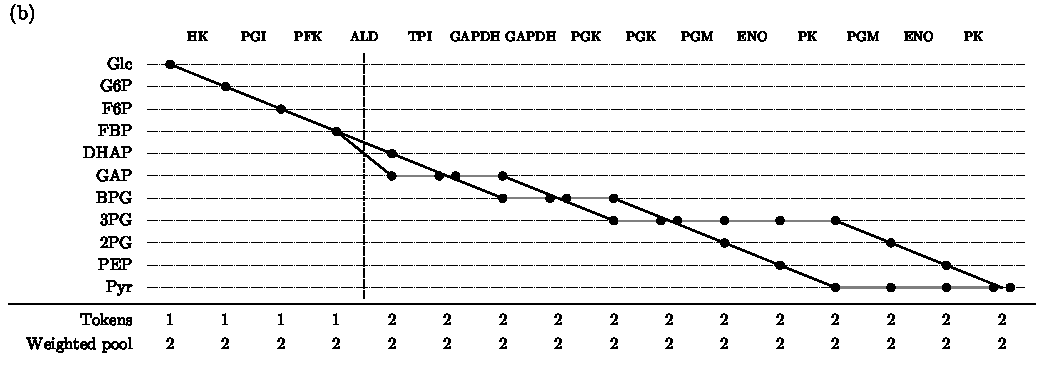
\includegraphics[width=16.4cm]{Figure/glycolysis_replay.pdf}};
\end{tikzpicture}
\endgroup

    \caption{Conserved pools and pathway realizability in reduced \texttt{KEGG} glycolysis (\texttt{M00001}). \textbf{(a)}~Bipartite network retaining polyphosphate and the ferredoxin bypass (dots: carbons, circled P: phosphate). \textbf{(b)}~Token markings along the certified 15-step conversion of one glucose to two pyruvates (single dot: one token; ringed dot: two tokens). Black lines trace consumed intermediates, gray lines carry unchanged pools, column headers name enzymes, and the dashed line marks aldolase cleavage. Shaded rows indicate hexoses, with pool weights $w$ on the right. Bottom rows trace total carbohydrate tokens and the invariant weighted pool ($2\times\text{hexoses} + 1\times\text{trioses} = 2$).}
    \label{fig:glycolysis}
\end{figure}

This incidence representation resolves information typically lost under net stoichiometric reduction (Fig.~\ref{fig:representation}). Eliminating shared polyphosphate from the reaction complexes of \texttt{R02189} leaves net stoichiometry $\mathbf S$, its nullspace, and its conservation laws unchanged ($\mathbf S_{\mathrm{retained}} = \mathbf S_{\mathrm{cancelled}}$). Yet this reduction alters the reaction topology, reducing complex count from 16 to 14, linkage classes from four to three, and deficiency from one to zero. Furthermore, net reduction destroys catalytic gating: the reduced reaction fires freely without polyphosphate, whereas explicit incidence correctly blocks firing until polyphosphate is supplied. Explicit reactant-product incidences thus enforce physical cofactor requirements discarded by net matrices.

Restoring currency metabolites (ATP, ADP, $\text{NAD}^+$, NADH, $\text{P}_i$, and $\text{PP}_i$) yields the complete 24-species metabolic network. Supplied solely with glucose, hexokinase cannot fire due to ATP depletion, and exhaustive search certifies that the pathway is unrealizable. The reduced model establishes topological feasibility of intermediate conversions, whereas full pathway execution requires balancing cofactor regeneration and energy charge (detailed with inventory controls in Supplementary Section~\ref{supp:si:kegg}).

\begin{figure}[!htbp]
\centering
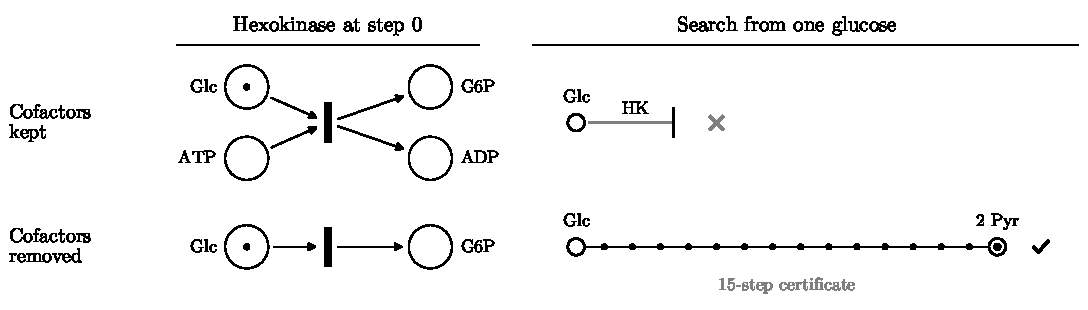
\includegraphics[width=\linewidth]{Figure/representation_sensitivity.pdf}
\caption{Sensitivity of structural invariants and pathway realizability to participant retention and currency omission. \textbf{(a)}~Reaction \texttt{R02189} with shared polyphosphate retained versus eliminated in net stoichiometry. \textbf{(b)}~Petri-net enabling under zero versus one polyphosphate token (check: enabled, cross: blocked). \textbf{(c)}~Prescribed glycolytic flux from one glucose under retained versus removed currency metabolites. Left: hexokinase (\texttt{R01786}) at step 0. Right: pathway reachability from initial glucose (open circle) through intermediate steps (dots) to two pyruvates (ringed dot).}\label{fig:representation}
\end{figure}

\subsection{Carbon conservation and precursor requirements in formose networks}
\label{sec:usecase_expand}

The formose reaction, in which formaldehyde condenses to a mixture of sugars~\cite{butlerov1861formose}, gives a rule-generated counterpart to the curated \texttt{KEGG} modules. Starting from formaldehyde and glycolaldehyde, four rules for aldol addition, retro-aldol cleavage, and reversible keto-enol tautomerization generate 37 species and 44 reactions after four iterations. Median cumulative generation time with the native \texttt{SynReactor} DPO controller is \DpoNativeFourSeconds~s across 20 timed runs after three warm-ups, and the network reaches species containing ten carbon atoms. The iteration count is a rule-expansion depth, not physical reaction time. The network has 54 complexes, 17 linkage classes, rank 36, and deficiency one.

Matched expansions in \texttt{M{\O}D}~1.0.0.75~\cite{andersen2016mod} and \texttt{MolFoundry}~0.1.11~\cite{friedrichs2026molfoundry} independently validate network generation. At six iterations, all three tools yield identical sets of 10\,572 species and 11\,239 stoichiometric reactions. Median cumulative generation times are \DpoNativeSixSeconds~s for native \texttt{SynReactor} DPO, \DpoModSixSeconds~s for \texttt{M{\O}D}, and \DpoMolfoundrySixSeconds~s for \texttt{MolFoundry}. Table~\ref{supp:tab:formose_dpo_comparison} gives per-depth results and resource limits. These measurements include rule and seed compilation and network construction on one logical CPU. Fig.~\ref{fig:formose_dpo_runtime}a shows network growth across the same six expansion depths, and Fig.~\ref{fig:formose_dpo_runtime}b shows the 20 individual runtime measurements, medians, and interquartile ranges. These are full API runtimes, including Python-side rule preparation and network construction for \synkit; they do not isolate native kernel execution.

\begin{figure}[!htbp]
\centering
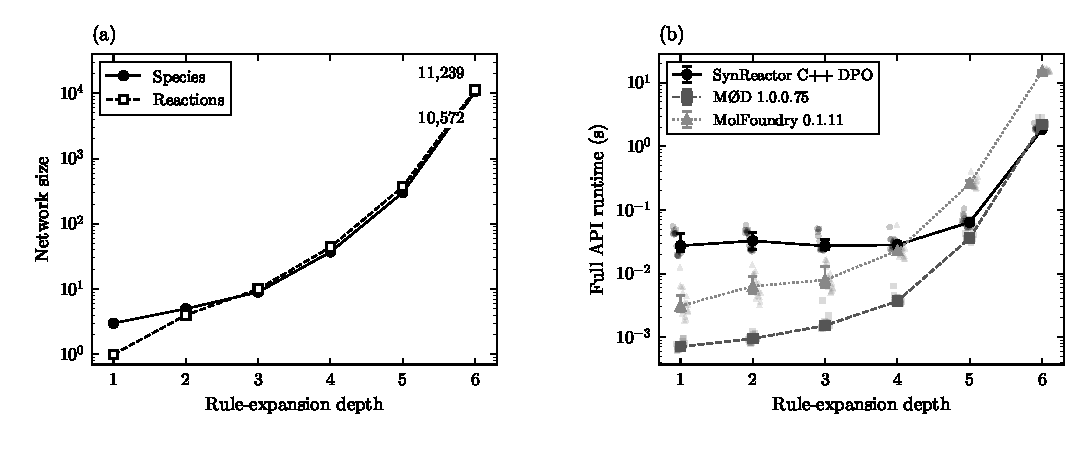
\includegraphics[width=\linewidth]{Figure/formose_dpo.pdf}
\caption{Formose network growth and full API runtime. \textbf{(a)}~Species and directed stoichiometric reactions across six rule-expansion depths; all three tools generate identical sets. \textbf{(b)}~Full API runtime of native \texttt{SynReactor} DPO, \texttt{M{\O}D}, and \texttt{MolFoundry}. Faint points show 20 timed runs per tool and depth after three warm-ups, large markers show medians, and error bars span the first and third quartiles. Points are offset horizontally for visibility. Times include per-call rule and seed preparation and network construction; imports, engine warm-up, and independent identity audits are excluded. Both panels use logarithmic vertical axes.}
\label{fig:formose_dpo_runtime}
\end{figure}

The four-iteration network's one-dimensional left nullspace yields a positive primitive conservation vector. Comparing its coefficients with carbon counts from the molecular graphs gives exact agreement for all 37 species (Fig.~\ref{fig:formose}). This is a consistency check between generated stoichiometry and molecular structures. Within this carbohydrate-only rule set, elemental counts can be proportional, but the result does not show that stoichiometry uniquely identifies elemental composition in general.

\begin{figure}[!htbp]
    \centering
    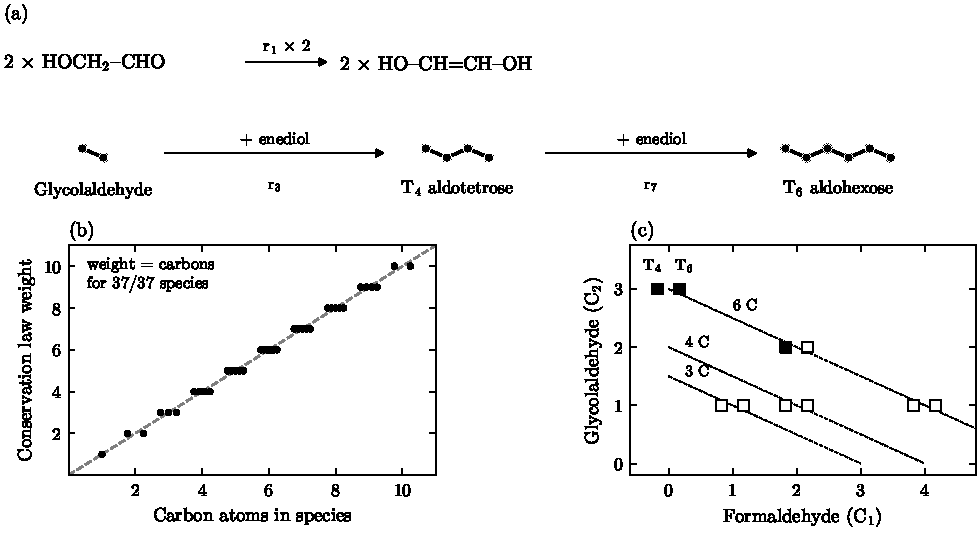
\includegraphics[width=\linewidth]{Figure/formose.pdf}
    \caption{Carbon conservation and precursor-dependent pathway realizability in the generated formose network. \textbf{(a)}~Target hexose route requiring three glycolaldehyde precursors via two enolizations ($r_1$) and two aldol additions ($r_3$, $r_7$), each addition consuming one enediol. \textbf{(b)}~Weights of the single conservation law against carbon atoms per species. They agree for all 37 species, which confirms that the generated reactions conserve carbon (points jittered horizontally, dashed line: $y=x$). \textbf{(c)}~Five initial inventories by formaldehyde and glycolaldehyde count, with dashed lines joining inventories of equal total carbon. The left and right squares of each inventory refer to the tetrose ($T_4$) and hexose ($T_6$) routes, filled when a certificate is verified and open when exhaustive search fails. Inventories with six carbon atoms differ in which routes they can supply.}
    \label{fig:formose}
\end{figure}

Qualitative search reaches representative tetrose and hexose targets from the two seed species, but realizability distinguishes inventories that share the same total carbon (Fig.~\ref{fig:formose}c). With four formaldehyde and one glycolaldehyde molecule, neither selected route is realizable. With two of each precursor, the tetrose route is realizable but the hexose route is not. With three glycolaldehyde molecules, both are. Each of these inventories contains six carbon atoms. The selected routes therefore require suitable precursor multiplicities as well as a sufficient carbon budget. \texttt{MolFoundry} independently agrees on all ten route--inventory decisions, and all three positive firing certificates pass independent replay. These results concern fixed reaction multisets in the generated network, and they do not establish unrestricted target unreachability or experimental synthetic feasibility. Supplementary Section~\ref{supp:sec:si_case_formose} gives the route definitions and initial pools.

\section{Conclusions}
\label{sec:discussion}

The CRN submodule of \synkit analyzes conserved pools, CRNT properties, and pathway realizability on one reaction representation that keeps reactant and product incidences separate. In the case studies, three modeling choices changed the answers. Cancelling shared polyphosphate preserved the net stoichiometric matrix but lowered deficiency and removed the donor requirement. Removing currency metabolites turned an exhaustively unrealizable glucose-to-pyruvate flux into a 15-step certificate. In the formose network, inventories with equal carbon differed in which routes they could supply. Conservation laws are therefore necessary, but not sufficient, evidence that a pathway can run from a given inventory.

Participant retention, cofactor boundaries, and initial inventories should thus be reported as model assumptions. \synkit supports this with exact rational arithmetic, explicit \texttt{inconclusive} outcomes, and independently replayable certificates, validated against \texttt{CRNT4SBML}, \texttt{BioModels} round trips, and \texttt{M\O D} and \texttt{MolFoundry} expansions.

\label{sec:limitations}
These analyses concern enabling and finite-inventory realizability in the discrete model, not reaction rates, concentrations, thermodynamic driving forces, or in vivo activity. Realizability is decided for a requested reaction multiset rather than for any route to a target, and multistationarity criteria beyond deficiency are not implemented. Exact enumeration can grow combinatorially, \texttt{SBML} exchange covers Core reaction structure only, and the generation benchmark includes Python-side rule preparation.

Future work will reduce Python/C++ transfer overhead, report resource use during exact enumeration, and add multistationarity criteria beyond deficiency. Coupling firing certificates with reaction free energies ($\Delta_r G$) and with constraint-based and kinetic tools would connect finite-inventory checks to quantitative models.

\vspace{1em}
\section*{Availability and requirements}
\begin{itemize}[leftmargin=*,label={},itemsep=0pt]
\item \textbf{Project name:} \synkit (CRN submodule)
\item \textbf{Project home page:} \href{https://github.com/TieuLongPhan/SynKit}{github.com/TieuLongPhan/SynKit}
\item \textbf{Software version:} \synkit~1.6.5~\cite{synkit165release}
\item \textbf{Operating system(s):} Platform independent (Linux, macOS, Windows)
\item \textbf{Programming language:} Python, C++17, and C++20
\item \textbf{Other requirements:} Python~$\ge$~3.10, \texttt{NetworkX}~$\ge$~3.3, \texttt{NumPy}, \texttt{SciPy}, \texttt{RDKit}, Boost headers, CMake
\item \textbf{License:} MIT
\item \textbf{Any restrictions to use by non-academics:} None
\end{itemize}

\section*{List of abbreviations}
\noindent \textbf{ACR}: Absolute concentration robustness, \textbf{CRN}: Chemical reaction network, \textbf{CRNT}: Chemical reaction network theory, \textbf{DPO}: Double pushout, \textbf{EMP}: Embden--Meyerhof--Parnas, \textbf{FBA}: Flux balance analysis, \textbf{\texttt{KEGG}}: Kyoto Encyclopedia of Genes and Genomes, \textbf{\texttt{SBML}}: Systems Biology Markup Language, \textbf{\texttt{SMARTS}}: SMILES arbitrary target specification, \textbf{TCA}: Tricarboxylic acid, \textbf{WR}: Weakly reversible.

\section*{Declarations}

\subsection*{Ethics approval and consent to participate}
Not applicable.

\subsection*{Consent for publication}
Not applicable.


\subsection*{Availability of data and materials}
The CRN submodule is distributed with \synkit under the MIT License.
Source code is available on GitHub at \href{https://github.com/TieuLongPhan/SynKit}{github.com/TieuLongPhan/SynKit}~\cite{synkit165release}, and the reproducible analysis scripts are located in the \href{https://github.com/TieuLongPhan/SynKit/tree/main/Experiment/CRN}{\texttt{Experiment/CRN}} directory.
\texttt{KEGG}~\cite{kanehisa2025kegg} pathways remain subject to \texttt{KEGG} terms, and \texttt{BioModels} entries are distributed under the CC0 1.0 Public Domain Dedication.

\subsection*{Use of generative AI}
Claude Opus (Anthropic) was used for language editing and TikZ figure formatting. The authors reviewed, verified, and take full responsibility for all manuscript content.

\subsection*{Competing interests}
The authors declare that they have no competing interests.

\subsection*{Funding}
This project has received funding from the European Union's Horizon Europe
Doctoral Network programme under the Marie-Sk{\l}odowska-Curie grant agreement
No~101072930 (TACsy, Training Alliance for Computational systems chemistry).
Views and opinions expressed are however those of the author(s) only and do not necessarily reflect those of the European Union. Neither the European Union nor the granting authority can be held responsible for them.

\subsection*{Authors' contributions}
Author contributions are reported using the CRediT taxonomy. \textbf{T.-A.P.}: Software, Validation, Writing (original draft), Writing (review and editing). \textbf{T.-L.P.}: Conceptualization, Methodology, Software, Validation, Writing (original draft), Writing (review and editing). Both authors read and approved the final manuscript.

\subsection*{Acknowledgements}
Not applicable.

% Bibliography
\bibliography{refs}

\end{document}
